\documentclass[12pt, a4paper]{scrartcl}

% CONFIG
\newcommand{\exptitle}{Muon decay}       % long name of experiment 
\newcommand{\exptitleshort}{Myon} % short name of experiment
\newcommand{\expdate}{April 20 to 24, 2015}           % date of experiment
\newcommand{\exptutor}{Manfredi \textsc{Ronzani}}

% PACKAGES + MODIFICATIONS
\usepackage[english]{babel} %standard language stuff
\usepackage[T1]{fontenc}
\usepackage[utf8]{inputenc}
\usepackage{textgreek}

\usepackage[fleqn]{amsmath}  % math
\usepackage{amssymb}

\usepackage{graphicx} %graphics
\usepackage{float} 
\graphicspath{{../img/}}

\usepackage[automark,headsepline]{scrlayer-scrpage} %headings
\pagestyle{scrheadings}
\ihead{\exptitleshort}
\ohead{\pagemark}
\cfoot{}

\usepackage{hyperref}
\hypersetup{
    unicode=true,          % non-Latin characters in Acrobat’s bookmarks
    pdftoolbar=true,       % show Acrobat’s toolbar?
    pdfmenubar=true,       % show Acrobat’s menu?
    pdffitwindow=false,    % window fit to page when opened
    pdfstartview={FitH},   % fits the width of the page to the window
    pdfnewwindow=true,     % links in new window
    colorlinks=true,       % false: boxed links; true: colored links
    linkcolor=blue,       % color of internal links (change box color with linkbordercolor)
    citecolor=green,       % color of links to bibliography
    filecolor=magenta,     % color of file links
    urlcolor=blue          % color of external links
}

\usepackage[labelfont=bf]{caption} % bold captions

\usepackage{chngcntr} % change behaviour of counters in different environments
\counterwithin{figure}{section}  % number figures per section
\numberwithin{equation}{section} % number equations per section
\numberwithin{table}{section}    % number tables per section

\usepackage{enumerate} % better way to config enumerates

\setcounter{tocdepth}{2} % table of contents depth

\setlength{\parindent}{0pt} % no indent on new paragraph

\usepackage{pdfpages} % include pdf files

% NEW COMMANDS
\newcommand{\difd}{\mathrm{d}}
\DeclareMathOperator{\cov}{cov}
\DeclareMathOperator{\gaus}{gaus}

% DOCUMENT SETTINGS

\title{\exptitle}
\subtitle{Fortgeschrittenen-Praktikum 1}
\author{Moritz Bitterling und Benjamin Rottler \\ Universität Freiburg}
\date{\expdate}

% DOCUMENT
\begin{document}

\hypersetup{pageanchor=false} %stop page numbering (hyperref) to prevent for double page numers
\newcommand{\HRule}{\rule{\linewidth}{0.5mm}}
\begin{titlepage}
\begin{center}
  \textsc{\Large Fortgeschrittenen-Praktikum II}\\[0.5cm]
  \HRule \\[0.4cm]
  { \huge \bfseries \exptitle}\\
  \HRule \\[0.5cm]
  \large \expdate\\[0.5cm]  
  \begin{minipage}{0.4\textwidth}
    \begin{flushleft} \large
      Moritz \\ \textsc{Bitterling}
    \end{flushleft}
  \end{minipage}
  \hfill
  \begin{minipage}{0.4\textwidth}
    \begin{flushright} \large
      Benjamin \\ \textsc{Rottler}
    \end{flushright}
  \end{minipage}
  \\[1cm]
  \large 
  Betreuer: \exptutor \\[3cm]
  
\includegraphics[height=8cm]{../../img/logo_uni.pdf}
  \vfill
  \normalsize
  \textsc{Institut für Mathematik und Physik} \\
  \textsc{Albert-Ludwigs-Universität} \\
  \textsc{Freiburg im Breisgau}
\end{center}
\end{titlepage}
\thispagestyle{empty}

\newpage
All calculations in this protocol were performed either with Python 3.4 using the following libraries
\begin{itemize}
  \item PyROOT (\url{http://root.cern.ch/drupal/content/pyroot})
  \item NumPy (\url{http://www.numpy.org/})
\end{itemize}
All graphics were drawn with Inkscape (\url{http://www.inkscape.org})\\[\baselineskip]
The python-scripts, \LaTeX-scripts and svg-graphics can be accessed online under
\url{https://github.com/Bigben37/FP2/tree/master/0420-Myon}.
\thispagestyle{empty}

\newpage
\tableofcontents
\thispagestyle{empty}

\newpage
\hypersetup{pageanchor=true} %start page numbering again
\setcounter{page}{1} %set to page 1

\section{Aim of the experiment}
mass + decay time of myon \\
weak 
\section{Physical Principles}
\subsection{Cosmic radiation}
Primary/Secendary radiation
\subsection{Energy loss by ionization and excitation}
Bethe-Bloch
\subsection{Muon}
\subsubsection{Muon decay}
\label{sub:decay}
\begin{equation}
	\frac{\difd N}{\difd t} = - \lambda N
\end{equation}
\begin{equation}
    \Rightarrow N(t) = N_0 e^{-\lambda t}
\end{equation}
\begin{equation}
    \tau := \frac{\left<t\right>}{\int_0^\infty N(t) \difd t} = 
    \frac{\int_0^\infty t e^{-\lambda t} \difd t}{\int_0^\infty e^{-\lambda t} \difd t} = 
    \frac{\frac{1}{\lambda^2}}{\frac{1}{\lambda}} = \frac{1}{\lambda}
\end{equation}
\subsection{V-A-Theory}
\section{Experimental setup}
\begin{figure}[H]
        \centering
        \def\svgwidth{0.95\textwidth}
       \input{../img/aufbau.pdf_tex}
        \caption{Experimental setup for the measurement of energy and decay time of cosmic muons.
        Muons are detected in a tank (filled with a scintillating fluid), causing flashes of light while flying through.
        The amount of light emitted is determined with photomultipliers,
        their signal then sent to a system of evaluating
        devices and recorded by multi channel analyzers.}
        \label{img:setup}
\end{figure}
\autoref{img:setup} shows the setup that was used in the experiment.
Its main part is a big metal tank filled with 470\,l of a liquid scintillator.
The flashes of light which are caused by the muons when they travel through the scintillator
are measured with two photomultipliers located at the edges of the cylindrical tank (PMl and PMr).
The signal from the two photomultipliers is then amplified with two \emph{linear amplifiers}.
The gain of the amplifiers is set to 2.
From these amplifiers, the signal goes into \emph{discriminators}.
They only let pass signals with an amplitude exceeding an adjustable threshold.
This threshold is set to a value which lets pass about 1000 pulses per second for each scintillator,
in order to cut off underground noise but also to let through enough desired muon signals.
The output signal of the discriminators is a rectangular pulse of about 50\,ns length and -1.0\,V amplitude.
\autoref{img:pmladisc} shows a pulse from PMr (yellow), the amplified signal (blue)
and the output of the discriminator (pink).
\begin{figure}[H]
\begin{center}
  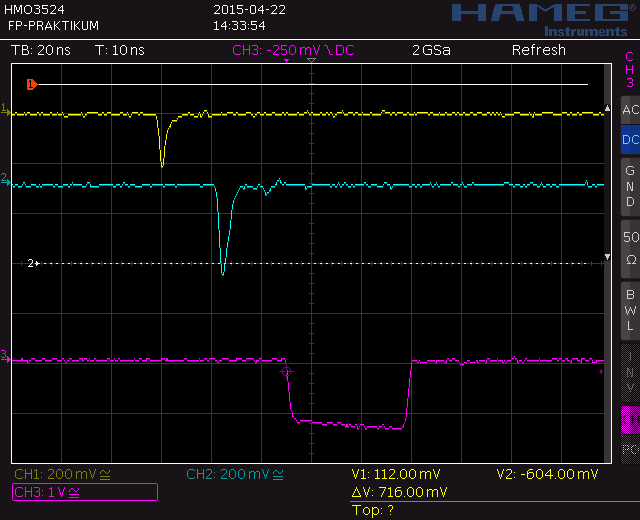
\includegraphics[width=0.5\textwidth]{../img/S0011.PNG}
  \caption{A muon passing through the scintillator causes a pulse of the photomultiplier PMr (yellow),
  the signal is then amplified (blue) and passes the discriminator
  which provides a rectangular output signal (pink).}
  \label{img:pmladisc}
\end{center}
\end{figure} 
The signals of the two discriminators are collected in a \emph{coincidence unit} (AND I).
The output signal of the coincidence unit is also a digital pulse like the one of the discriminators
and it is triggered only if two signals from the discriminators reach its inputs simultaneously.
This configuration again blocks a lot of undesired underground signals,
since it is assumed that a muon passing the tank will generate a signal in both photomultipliers at once.
A counter (Z I) after the coincidence unit permits the determination of the number of coinciding signals
over a specific period.
\autoref{img:discdiscandI} shows a sample of those signals
(the signal from the discriminators in yellow and blue and the output of the coincidence unit in pink).
\begin{figure}[H]
\begin{center}
  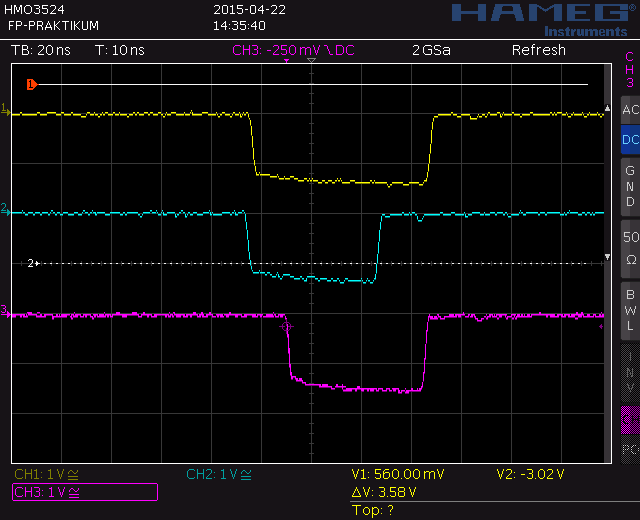
\includegraphics[width=0.5\textwidth]{../img/S0012.PNG}
  \caption{Coinciding signals from the discriminators (yellow and blue) create a pulse
  of the coincidence unit AND I (pink).}
  \label{img:discdiscandI}
\end{center}
\end{figure}
In order to determine the energy of the muon, the analog signals of the linear amplifiers
also take a second way in the circuit:
The signals are \emph{added} and then delayed by 170\,ns in a \emph{delay generator}
(to await analysis of the signals in a different part of the setup, this will become clear later).
\autoref{img:lalaadddel} shows the described signals, from the amplifiers in yellow and blue,
the sum signal in pink and the delayed signal in green.
\begin{figure}[H]
\begin{center}
  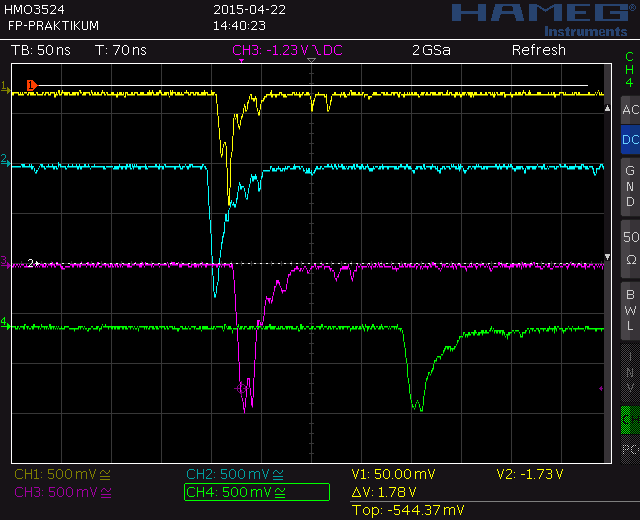
\includegraphics[width=0.5\textwidth]{../img/S0013.PNG}
  \caption{A muon causes peaks after the amplifiers (yellow and blue). The peaks are added (pink)
  and delayed (green).}
  \label{img:lalaadddel}
\end{center}
\end{figure}
After the delay generator, the signal goes over a \emph{capacitor} (to block the constant component of the signal)
and into a \emph{linear gate}.
The control signal for the gate comes from a different part of the setup and gets triggered
if the approach of a muon has been detected in the scintillating tank.
\autoref{img:delcapgate} shows a signal before the capacitor (yellow), after it (blue),
the control signal for the linear gate (pink) and the output signal of the gate (green).
On the figure it can be seen clearly that a signal can only pass the gate if it is open:
The first peak of the blue signal can not pass, but the second runs through the gate,
since it is opened by the pink pulse.
The additional two small peaks of the green signal occur due to the opening and closing of the gate
and constitute the main cause of the \emph{pedestal} which is measured in the course of the experiment.
\emph{Pedestal} refers to the nonzero amplitude coming from the linear gate after opening
even if there is no incoming signal.
\begin{figure}[H]
\begin{center}
  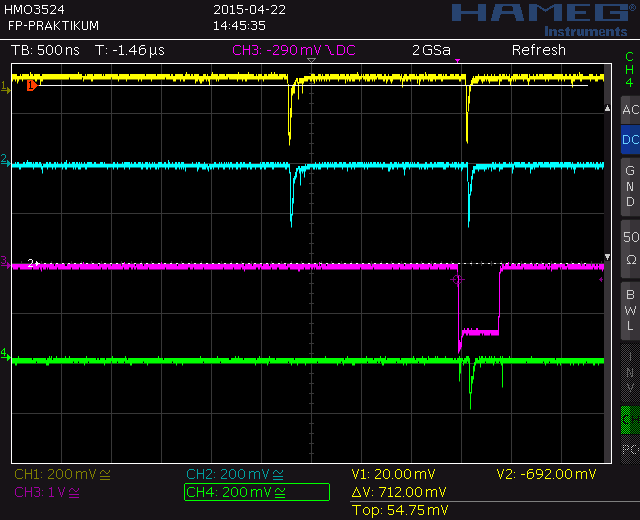
\includegraphics[width=0.5\textwidth]{../img/S0014.PNG}
  \caption{Signature of muon decay in the tank: The first peak is caused by the incoming muon,
  the second by the electron originating in the decay of the muon after 1.8\,\textmu s.
  The signals are measured before the capacitor (yellow) and after the capacitor (blue).
  The control signal for the linear gate is depicted in pink and the output of the linear gate in green.
  The first signal can not pass the gate because the control signal is not supplied.}
  \label{img:delcapgate}
\end{center}
\end{figure}
An \emph{attenuator} after the linear gate damps the signal.
The attenuation for the main measurement is -12\,dB in order not to overload the following \emph{shaping amplifier}
which shows nonlinear behaviour above an input signal of about 100\,mV.

\autoref{img:gateattshamp} shows the signal from the linear gate (yellow), the attenuated signal (blue) and
the signal from the shaping amplifier (pink).
The shaping amplifier integrates and differentiates its input signal and yields an output signal
whose maximum amplitude is proportional to the charge of the input signal.

After the shaping amplifier a \emph{multi channel analyzer} ranks the pulses by their amplitude
and sends the data to a computer.

\begin{figure}[H]
\begin{center}
  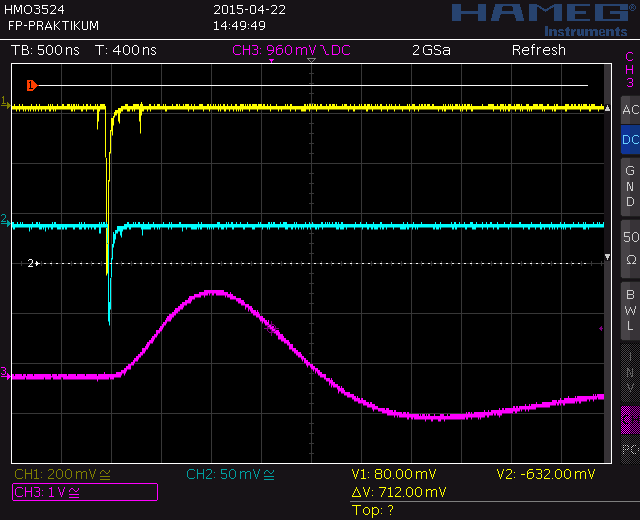
\includegraphics[width=0.5\textwidth]{../img/S0015.PNG}
  \caption{Signal from the linear gate (yellow), attenuated signal (blue) and signal after the shaping 
 amplifier (pink). The amplitude of this signal contains information about the energy of the muon.}
  \label{img:gateattshamp}
\end{center}
\end{figure}

To generate the control signal for the linear gate, additional units are necessary:
Two more scintillators with photomultipliers over and under the tank (PMt and PMb)
detect the approach (and the flight through) of muons.
Here again two discriminators are used to block small signals.
The discriminator levels are set to values which lead to about 200 counts per second.
After the discriminators, the signal is delayed by 25\,ns to keep in time with the other components
of the setup.

\autoref{img:tdiscdel} shows a pulse of 
the photomultiplier over the tank (yellow), the signal after the discriminator (blue) and
the delayed signal.

\begin{figure}[H]
\begin{center}
  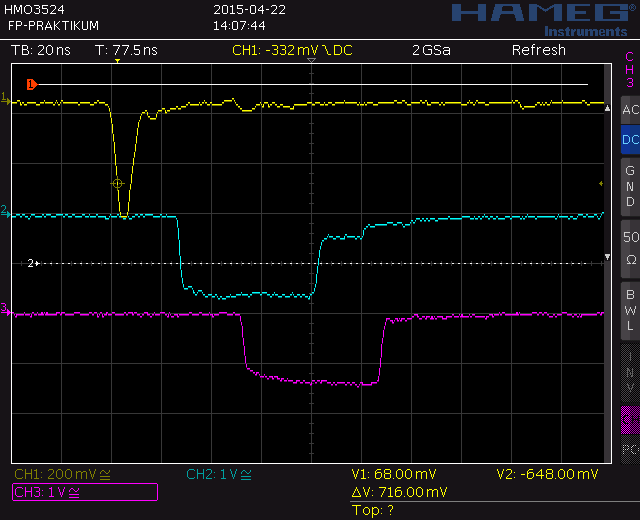
\includegraphics[width=0.5\textwidth]{../img/S0006.PNG}
  \caption{Signal from the photomultiplier over the tank (yellow), digital signal after the discriminator (blue)
  and delayed signal (pink).}
  \label{img:tdiscdel}
\end{center}
\end{figure}

The signal from the photomultiplier under the tank is processed the same way and
the signals from the two delay generators go into another coincidence unit (AND~II),
together with the output of AND~I. The inputs of AND~II can be switched off and on,
thus it can be defined which input conditions are necessary to trigger an output signal of AND~II.
The assignment of the inputs A, B and C can be seen on \autoref{img:setup}.
The counter Z~II counts the events after AND~II.
\autoref{img:discdiscandII} shows input (yellow and blue) and output signal (pink) of AND~II.

\begin{figure}[H]
\begin{center}
  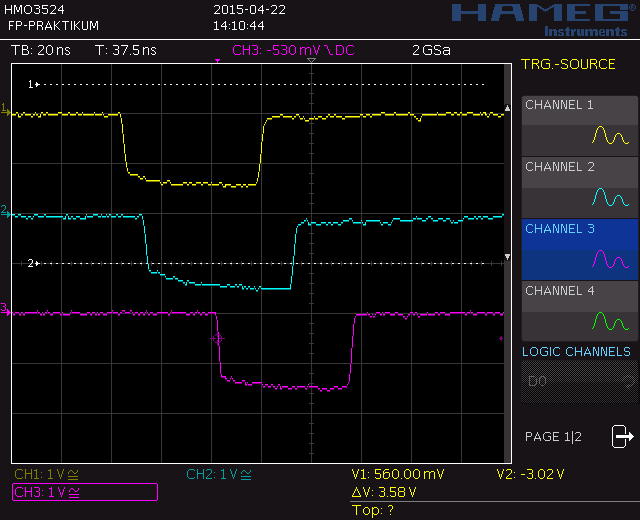
\includegraphics[width=0.5\textwidth]{../img/S0007.PNG}
  \caption{A muon flying through the tank causes two coinciding signals (yellow and blue) going
  into the coincidence unit AND II. The output signal is in pink.}
  \label{img:discdiscandII}
\end{center}
\end{figure}

The output signal of AND II is delayed by 500\,ns in a \emph{gate/delay generator}.
This delay is necessary to avoid the incorrect identification of a passing muon as a decaying muon
in a following section of the setup.
The gate/delay generator triggers the opening of a 7.5\,\textmu s wide window in the subsequent
\emph{timing unit}.
The signals are shown on \autoref{img:andIIgatetu}: The pulse after AND II in yellow,
the delayed pulse from the gate/delay generator in blue and the window of the timing unit in pink.

\begin{figure}[H]
\begin{center}
  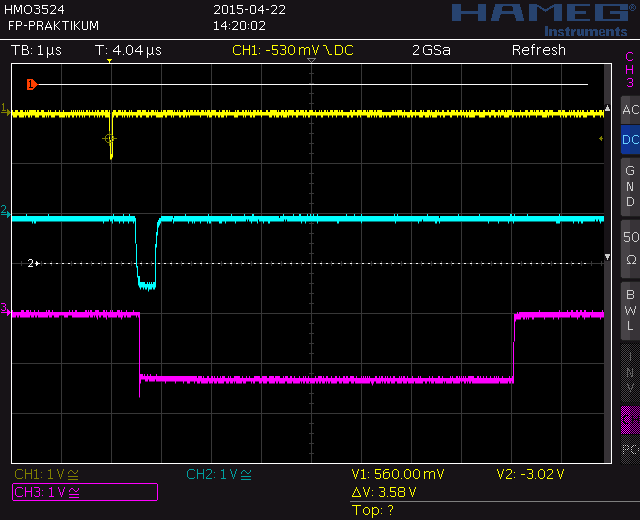
\includegraphics[width=0.5\textwidth]{../img/S0009.PNG}
  \caption{Pulse after the coincidence unit AND~II (yellow), delayed signal after the gate/delay generator (blue)
  and 7.5\,\textmu s-window of the timing unit (pink).}
  \label{img:andIIgatetu}
\end{center}
\end{figure}

The signal of the timing unit (which occurs once the intrusion of a muon in the tank is detected)
then goes into another coincidence unit AND~III (input A).
During the wide window of the timing unit the decay of the muon can cause a signal
of the coincidence unit AND~I. This signal also goes into AND~III
(yellow on \autoref{img:andItuIandIIItuII}).
After AND~III (pink),
another timing unit with a window of 400\,ns provides the opening signal for the linear gate (green).

For the flight through measurement it is possible to shortcut the gate/delay generator and the timing unit
and to pass the signal of AND~II directly into AND~III (input B).

Events of AND~III are counted with the counter Z~III.

\begin{figure}[H]
\begin{center}
  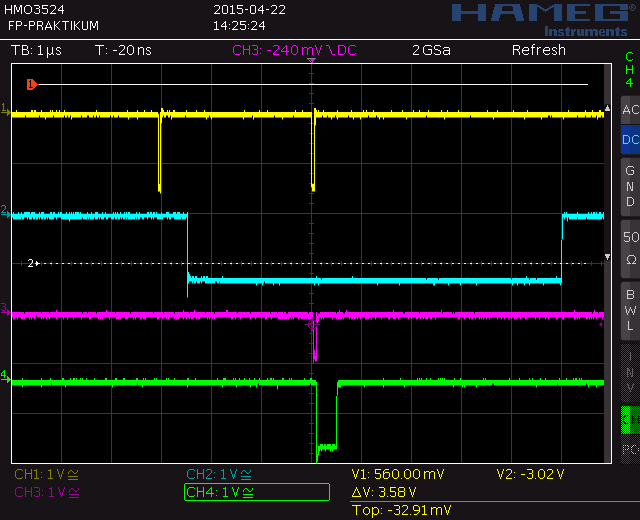
\includegraphics[width=0.5\textwidth]{../img/S0010.PNG}
  \caption{Creation of the control signal for the linear gate (green):
  The coincidence unit AND~I records two events (yellow), the first event arising from the intrusion
  of a muon in the tank. This triggers a wide window of the timing unit~I (blue) which
  allows the second pulse of AND~I due to the decay of the muon to pass through AND~III (pink).
  The signal of AND~III opens a window after the timing unit~II (green).}
  \label{img:andItuIandIIItuII}
\end{center}
\end{figure}

For the measurement of the decay time of muons a \emph{time to amplitude converter} is used.
It provides a signal whose amplitude is proportional to the time difference between a start and a stop signal.
The start signal is delivered by the coincidence unit AND~II when a muon enters the tank.
The stop signal comes from AND~III when a decay is recorded.
The output of the TAC goes into a multi channel analyzer which is connected to a computer.
The signals for and from the TAC are shown on \autoref{img:tac}.\\

To perform the time calibration of the TAC, a special device is provided to generate start and stop
pulses with adjustable time difference.\\

For the determination of the energy resolution of the setup a LED is integrated in the tank.
The LED is controlled with a pulse generator and a LED driver.


\begin{figure}[H]
\begin{center}
  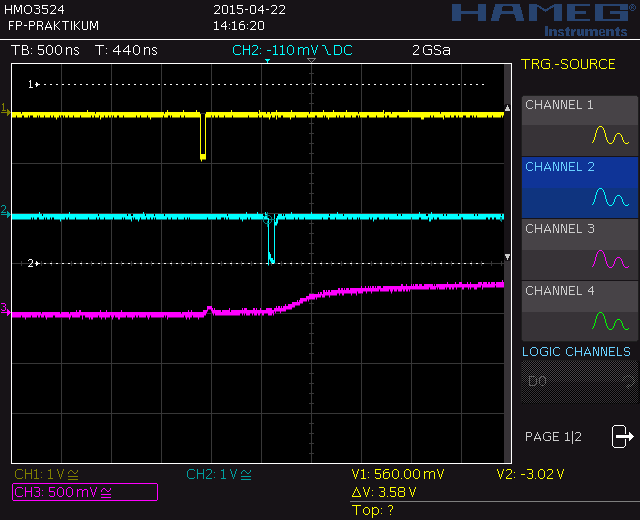
\includegraphics[width=0.5\textwidth]{../img/S0008.PNG}
  \caption{Signals at the time to amplitude converter: Start (yellow), stop (blue) and output (pink).}
  \label{img:tac}
\end{center}
\end{figure}

To verify the correct operation of the system after setting it up and during the days of the measurements,
the count rates of the four photomultipliers and the coincident events were monitored regularly.
\autoref{tab:countrates} shows the values that were determined after the successful completion of the setup.

\begin{table}[H]
\caption{Count rates at various configurations of the setup.}
\begin{center}
\begin{tabular}{|c||c|c|c|c|c|c|}
  \hline 
  					& counter	& AND I	& AND II	& AND III	& counts				& count rate\footnotemark/ s$^{-1}$			\\ \hline \hline
  PMr				& Z I		& A		& -			& -			& 141443/100\,s			& \textbf{1414\,$\pm$\,4}					\\ \hline
  PMl				& Z I		& B		& -			& -			& 78865/100\,s			& \textbf{789\,$\pm$\,3}					\\ \hline
  PMt				& Z II		& -		& A			& -			& 16640/100\,s			& \textbf{166.4\,$\pm$\,1.3}				\\ \hline
  PMb				& Z II		& -		& B			& -			& 17181/100\,s			& \textbf{171.8\,$\pm$\,1.3}				\\ \hline
  PMr \& PMl		& Z I		& A B	& -			& -			& 106649/1000\,s		& \textbf{106.7\,$\pm$\,0.3}				\\ \hline
  PMt \& PMb		& Z II		& -		& A B		& -			& 108/100\,s			& \textbf{1.08\,$\pm$\,0.10}				\\ \hline
  t \& r \& l		& Z III		& A B	& A	C		& B C		& 20990/1000\,s			& \textbf{20.99\,$\pm$\,0.14}				\\ \hline
  t \& b \& r \& l  & Z III		& A B	& A	B C		& B C		& 973/1000\,s			& \textbf{0.97\,$\pm$\,0.03}				\\ \hline
  decays			& Z III		& A B	& A	C		& A C		& 213/1000\,s			& \textbf{0.213\,$\pm$\,0.014}				\\ \hline
  underground\footnotemark		& Z III		& A B	& A	C		& A C		& 16/1000\,s			& \textbf{0.016\,$\pm$\,0.004}				\\ \hline
\end{tabular}
\end{center}
\label{tab:countrates}
\end{table}

\addtocounter{footnote}{-1}
\footnotetext{The errors were calculated with Gaussian uncertainty propagation,
assuming a Poisson distribution of the error on the number of counts (see section \ref{subsub:errorcountrate}).}
\addtocounter{footnote}{1}
\footnotetext{For the measurement of the underground, the gate/delay time was increased by a factor of 100.}	

\section{Experimental Procedure}


\subsection{Energy resolution: Photoelectronstatistics}
For the determination of the energy resolution of the setup, the LED in the tank is used.
\autoref{tab:conderes} shows the input conditions of the coincidence units during the measurements.
A pulse generator produces a periodic signal with a frequency of 5\,kHz.
The signal is delivered to a LED driving unit, where the intensity of the LED can be adjusted.
12~measurements with different intensities are conducted, in order to cover the whole energy range of the MCA.
The duration of each measurement is 1\,min.
For the three lowest intensities, the measuring time is increased to 6\,min, 3\,min and 2\,min to reduce the error
on the count rate.
Each measurement produces an energy spectrum on MCA\,I which is saved.

\begin{table}[H]
\caption{Active inputs of the coincidence units during measurement of the energy resolution of the setup.}
\begin{center}
\begin{tabular}{|c|c|}
  \hline
  coincidence unit	& active inputs	\\ \hline
  AND I				& A B			\\ \hline
  AND II			& -				\\ \hline
  AND III			& C				\\ \hline
 \end{tabular}
\end{center}
\label{tab:conderes}
\end{table}

\subsection{Energy calibration}

\subsubsection{Pedestal measurement}
\autoref{tab:condped} shows the state of the setup for the measurement of the pedestal.
Due to this wiring, the linear gate is opened each time a signal from PMt is delivered.
As only about every 8th event from PMt coincides with an event of PMr and PMl (\autoref{tab:countrates}),
in this configuration most likely no signal will pass the gate when it is opened.
Such events give rise to the pedestal, a large peak at the low end of the spectrum measured with MCA\,I.
After minimizing the pedestal with the offset screws on the delay generators, the pedestal is measured for
5\,min.

\begin{table}[H]
\caption{Active inputs of the coincidence units during measurement of the pedestal.}
\begin{center}
\begin{tabular}{|c|c|}
  \hline
  coincidence unit	& active inputs	\\ \hline
  AND I				& -				\\ \hline
  AND II			& A				\\ \hline
  AND III			& B				\\ \hline
 \end{tabular}
\end{center}
\label{tab:condped}
\end{table}

\subsubsection{Flight through spectrum}


\subsection{Time calibration}


\subsection{Underground measurement}

\subsection{\textbeta-spectrum and mean lifetime}


energycal
pedestal,flight through

timecal

underground

betaspectrum+lifetime

\section{Measurement results and evaluation}

\subsection{General remarks}
\subsubsection{Errors and count rate}
\label{subsub:errorcountrate}
The number $N$ of measurement events of a channel of the MCAs is Poisson distributed. Hence the error $s_N$  of $N$ events is:
\begin{equation}
  s_N = \sqrt{N}
\end{equation}

Not all measurements were done in the same amount of time, so we decided to normalize all measured data with the elapsed time $t$ to a 
count rate $n$. Consequently the error changes, too:
\begin{equation}
    n = \frac{N}{t}, \qquad s_n = \frac{s_N}{t}
\end{equation}
\subsubsection{Gaussian distribution}
For some fits we use the Gaussian distribution. The following convention will be used:
\begin{equation}
	\label{eq:gaus}
    \gaus(c;x,\sigma) = e^{-\frac{1}{2} \left( \frac{c-x}{\sigma} \right)^2}
\end{equation}
in which $\gaus(c;x,\sigma)$ is a function of $c$ with parameters $x$ (expectation value) and $\sigma$ (standard deviation).

\subsubsection{Rebinning}
\label{subsub:rebinning}
Sometimes there is too much noise in the spectrum to recognize a trend. In those cases $n$ successive $(x, y)$ tuples are averaged:
\begin{equation}
    \bar{x}_i = \frac{1}{n} \sum_{j=0}^{n-1} x_{ni+j}, \qquad \bar{y}_i = \frac{1}{n} \sum_{j=0}^{n-1} y_{ni+j}, \qquad i = 1, 2, \ldots, \frac{\#(x_i)}{n}
\end{equation}
where $(x_i, y_i)$ are the old values and $(\bar{x}_i, \bar{y}_i)$ are the new ones. $\#(x_i)$ is the number of old values.
The errors are calculated with error propagation:
\begin{equation}
    s_{\bar{x}_i} = \frac{1}{n} \sqrt{\sum_{j=0}^{n-1} s_{x_{ni+j}^2}}, \qquad s_{\bar{y}_i} = \frac{1}{n} \sqrt{\sum_{j=0}^{n-1} s_{y_{ni+j}^2}}
\end{equation}


\subsection{Energy resolution}
The spectra for the energy resolution measurement are fitted with a Gaussian distribution and a constant offset:
\begin{equation}
    n(c) = b + A \gaus(c;x,\sigma)
\end{equation}
An example fit is shown in \autoref{img:eres:400}. Ideally a line is expected, but because of the energy resolution it is blurred into a Gaussian 
distribution. The standard deviation $\sigma$ of the Gaussian distribution is a measure for the energy resolution. 
From \autoref{img:eres:multi} can be seen that with increasing channel number the energy resolution decreases. All fitted standard deviations are 
plotted against the expectation value of their respective Gaussian distributions (\autoref{img:eres:channels}).
\begin{figure}[H]
\begin{center}
  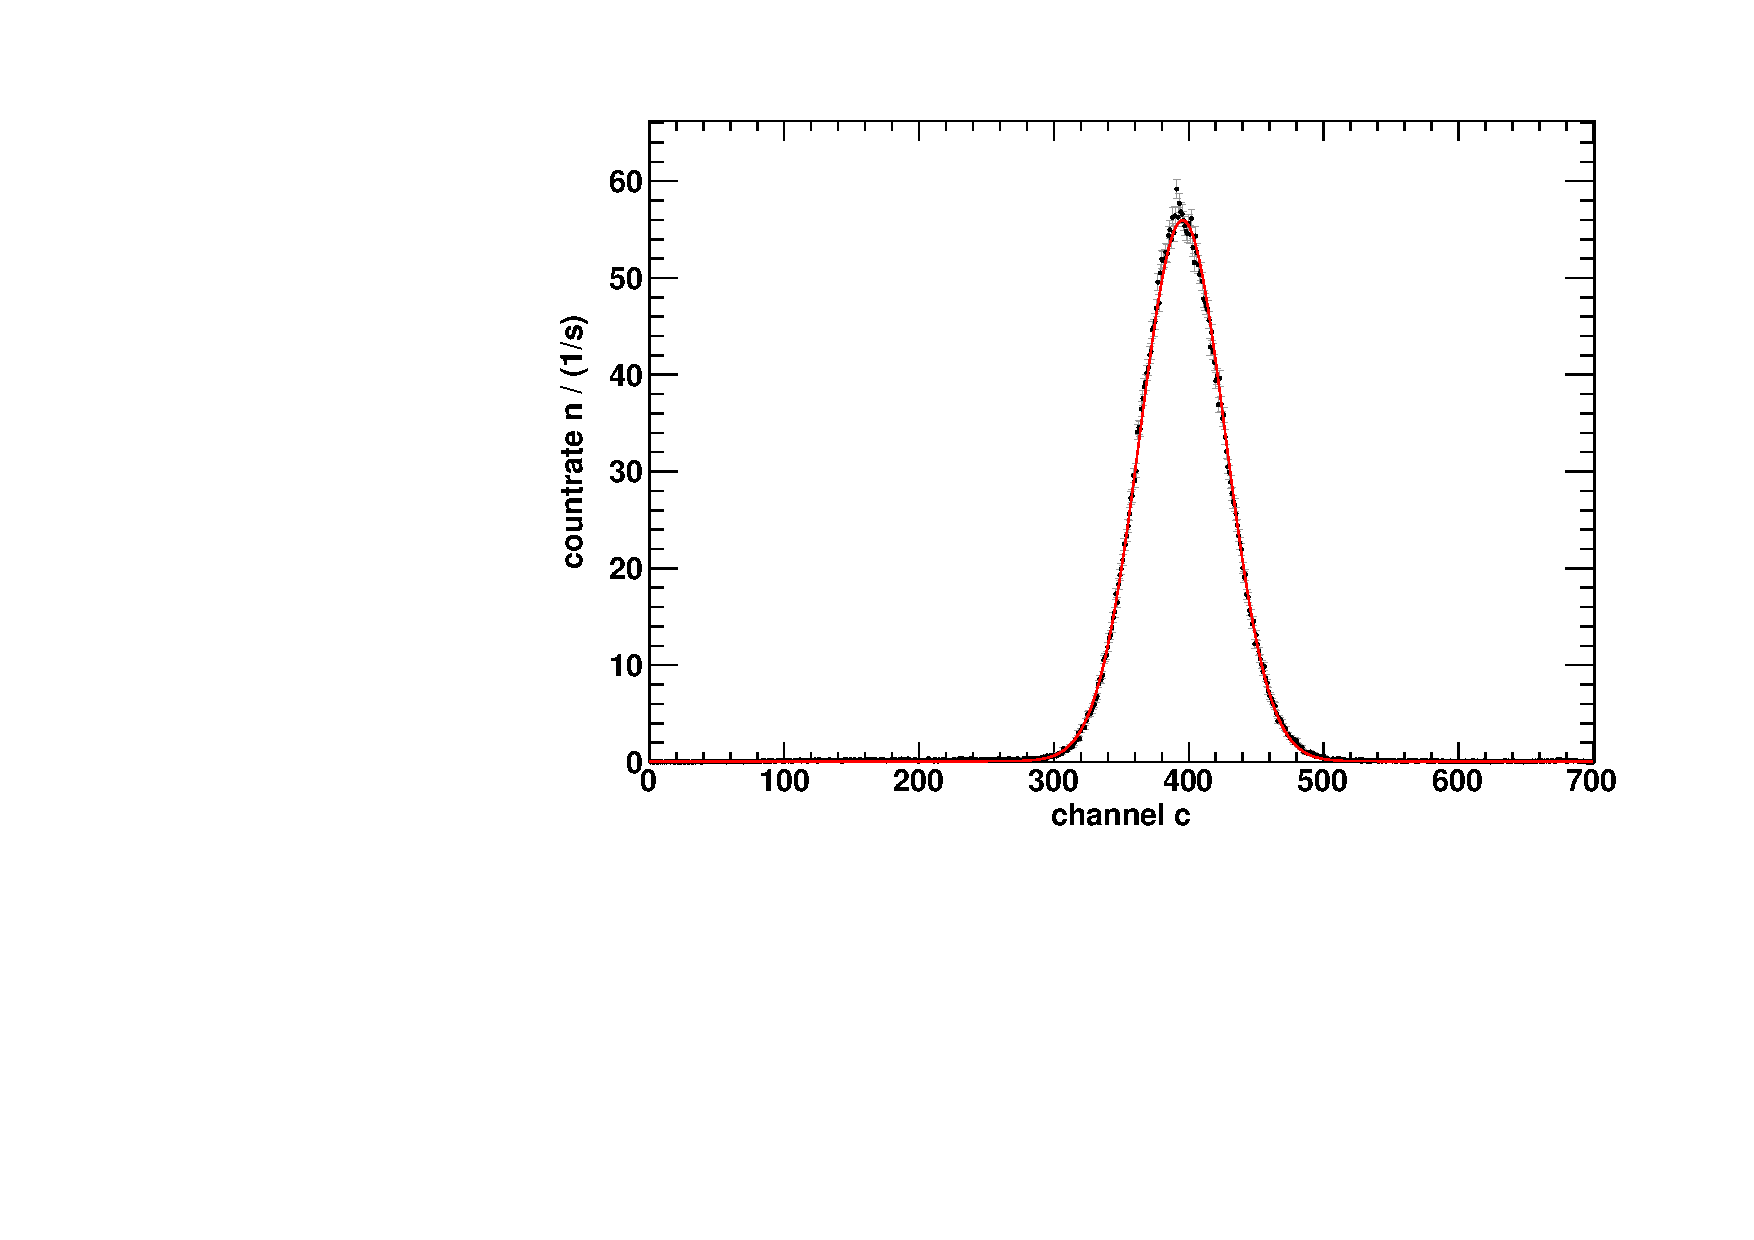
\includegraphics[width=\textwidth]{../img/energieaufloesung_400.pdf}
  \caption{Recorded and fitted spectrum of the LED flashing in the tank for one minute with medium intensity.}
  \label{img:eres:400}
\end{center}
\end{figure}

\begin{figure}[H]
\begin{center}
  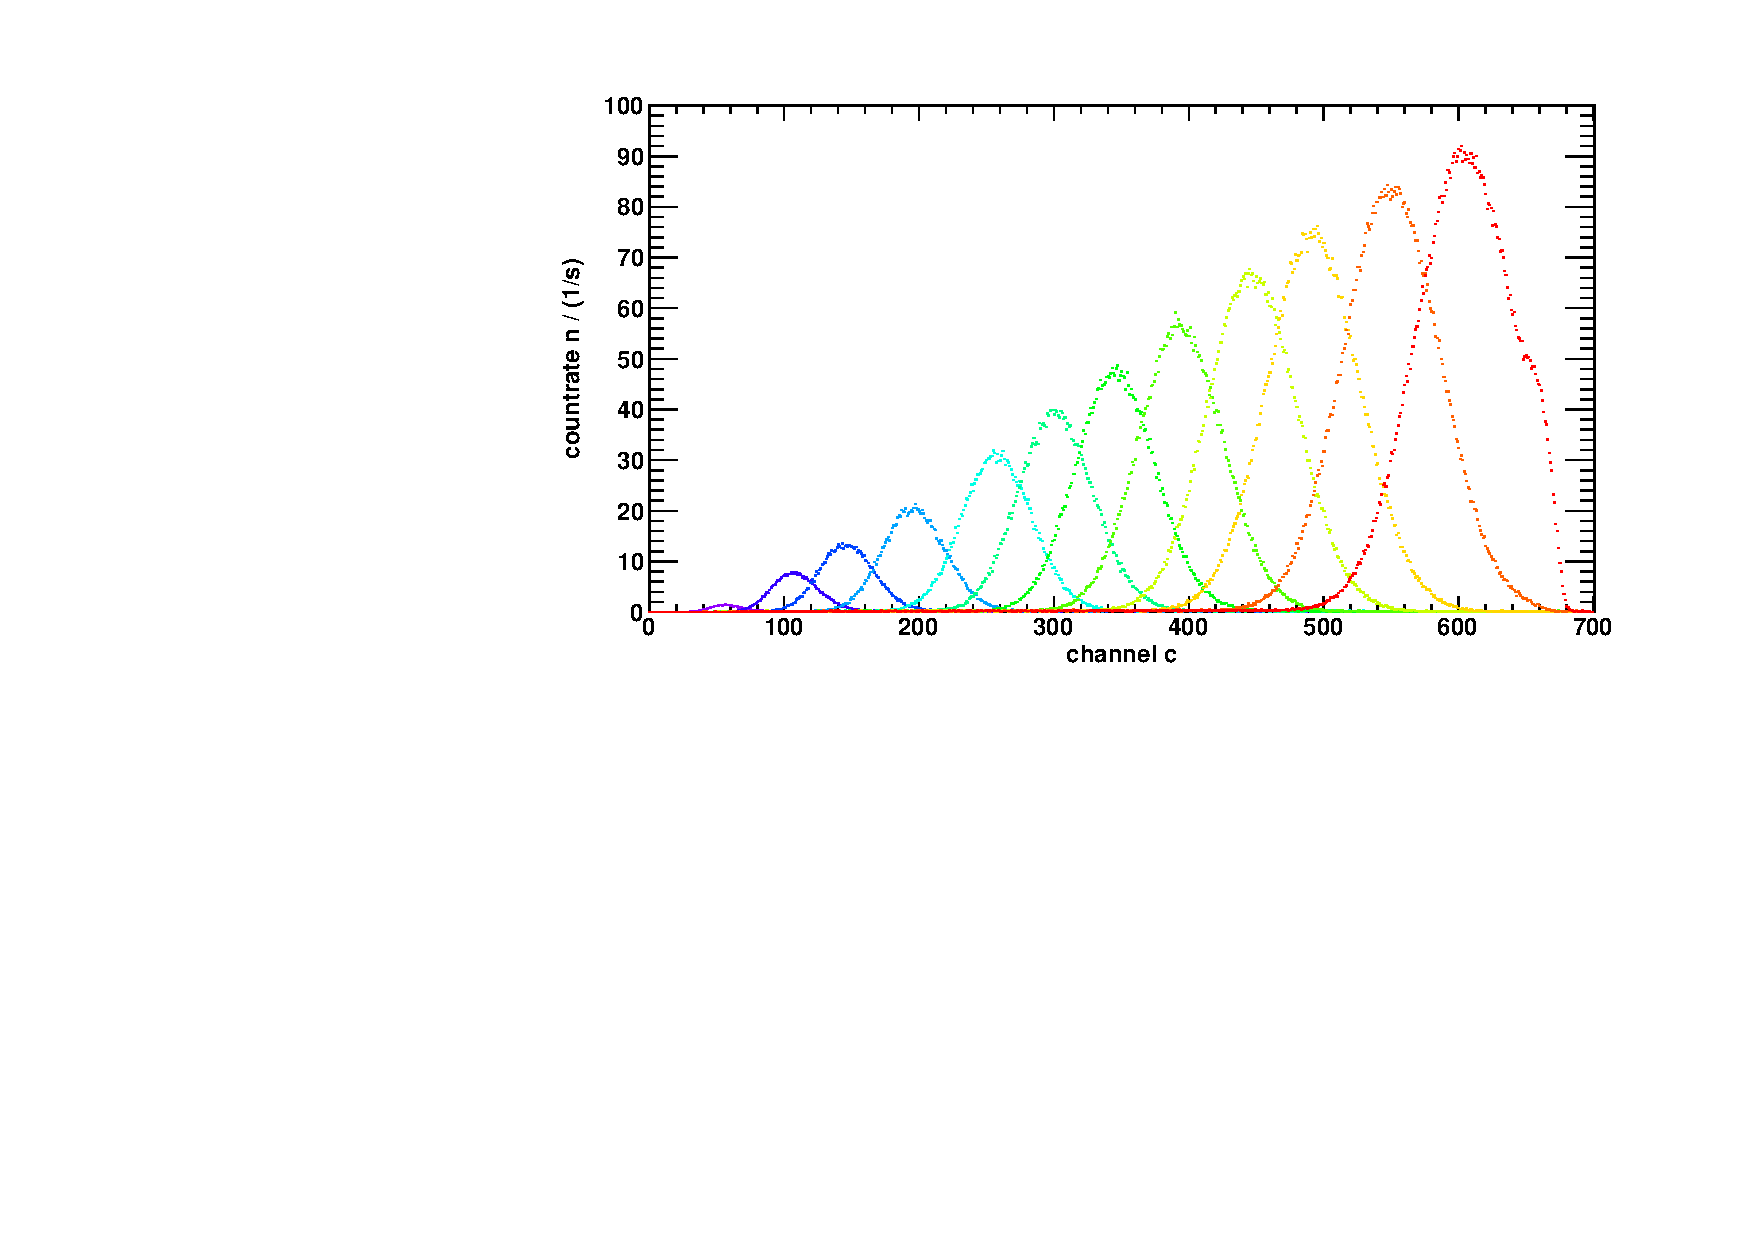
\includegraphics[width=\textwidth]{../img/energieaufloesung_multi.pdf}
  \caption{All measured energy spectra of the flashing LED in the tank.
  Raising the intensity of the LED increases the expectation value,
  the standard deviation (energy uncertainty) and the amplitude of the distributions.}
  \label{img:eres:multi}
\end{center}
\end{figure}


\begin{figure}[H]
\begin{center}
  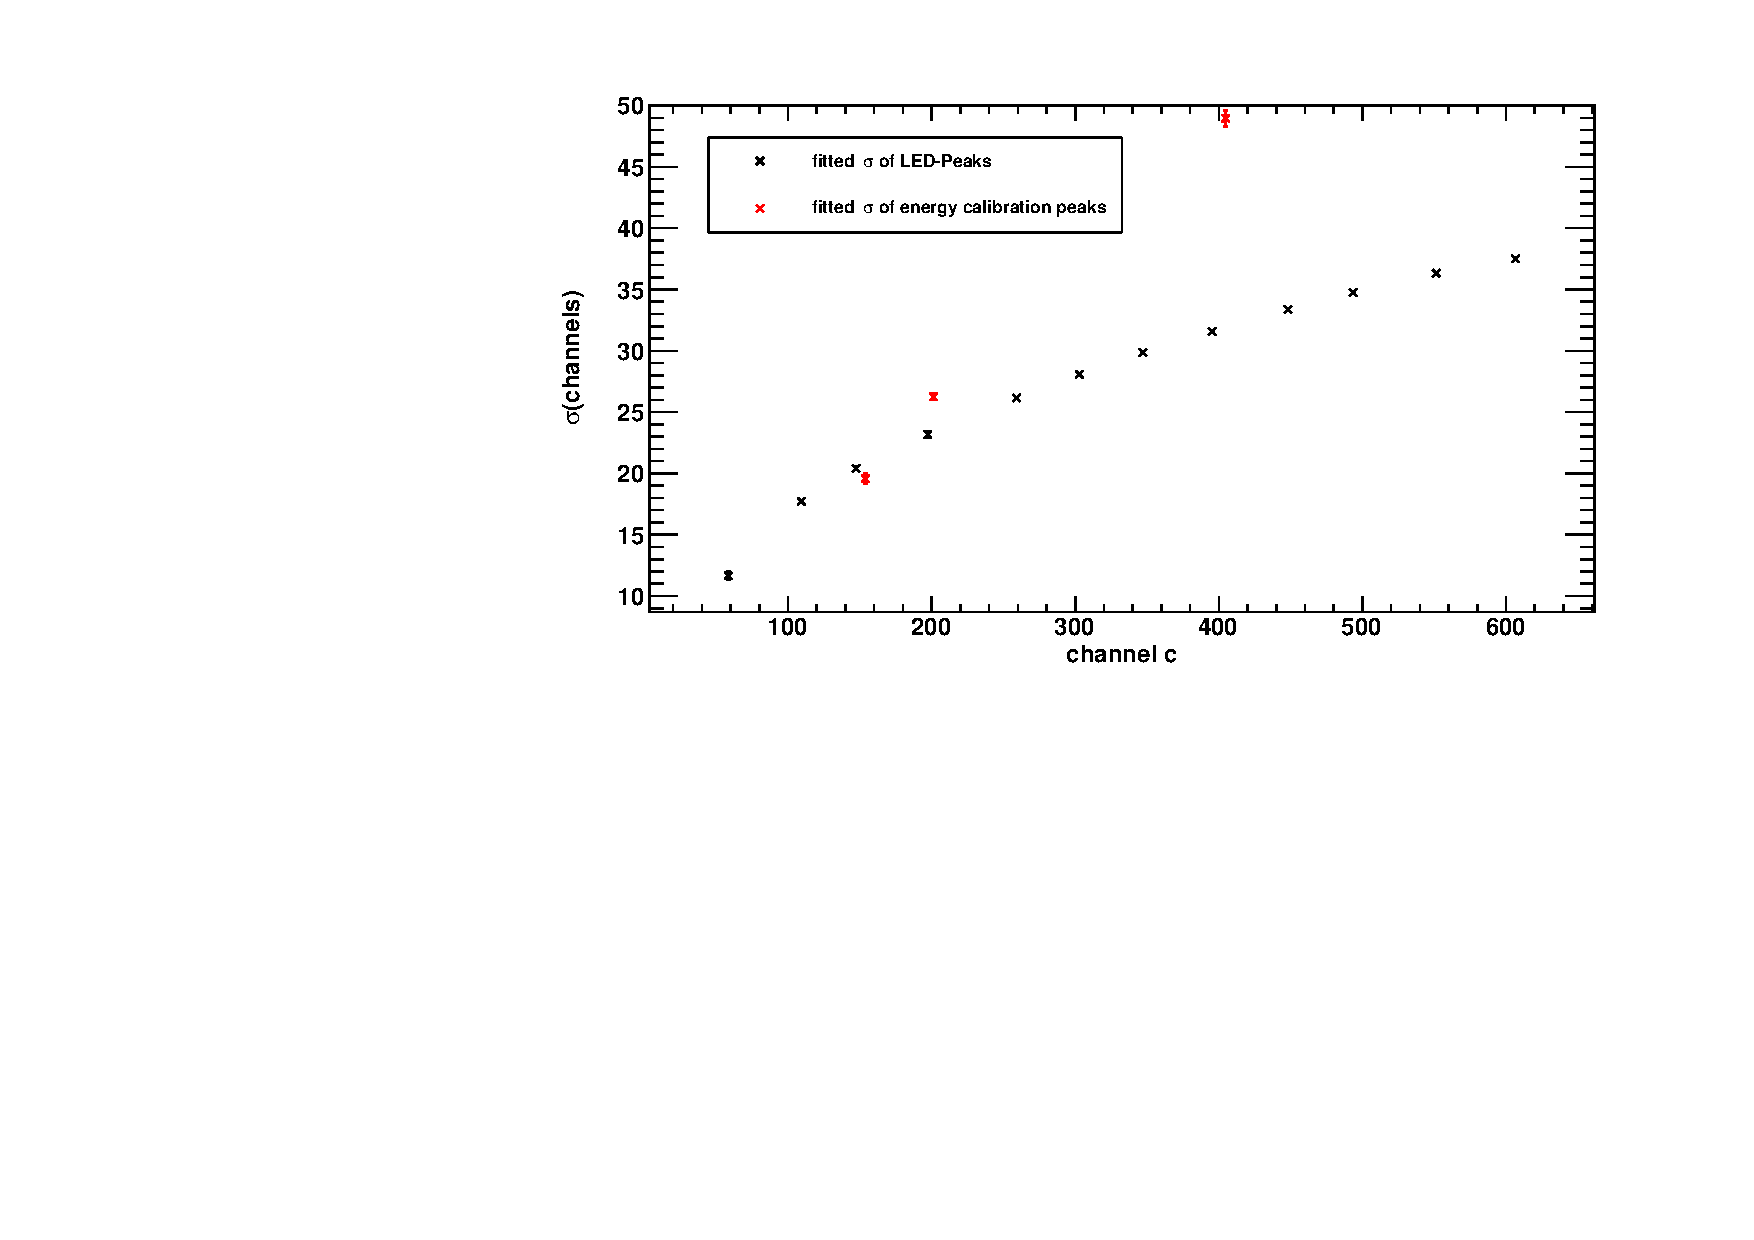
\includegraphics[width=\textwidth]{../img/energieaufloesung_channels+ecal.pdf}
  \caption{Fitted standard deviations plotted against the expectation value of their respective Gaussian distributions as seen in 
  \autoref{img:eres:multi}. The red points are the blurs of the flight through spectra (evaluated in section \ref{subsub:flightthroughspectra}).}
  \label{img:eres:channels}
\end{center}
\end{figure}

\subsection{Energy calibration}
For the energy calibration the pedestal measurement and flight through spectra are evaluated. Then the theoretical energies are calculated 
and those two datasets are plotted against each other.
\subsubsection{Pedestal}
The pedestal measurement produced a Gaussian distributed spectrum (\autoref{img:pedestal}).
\begin{figure}[H]
\begin{center}
  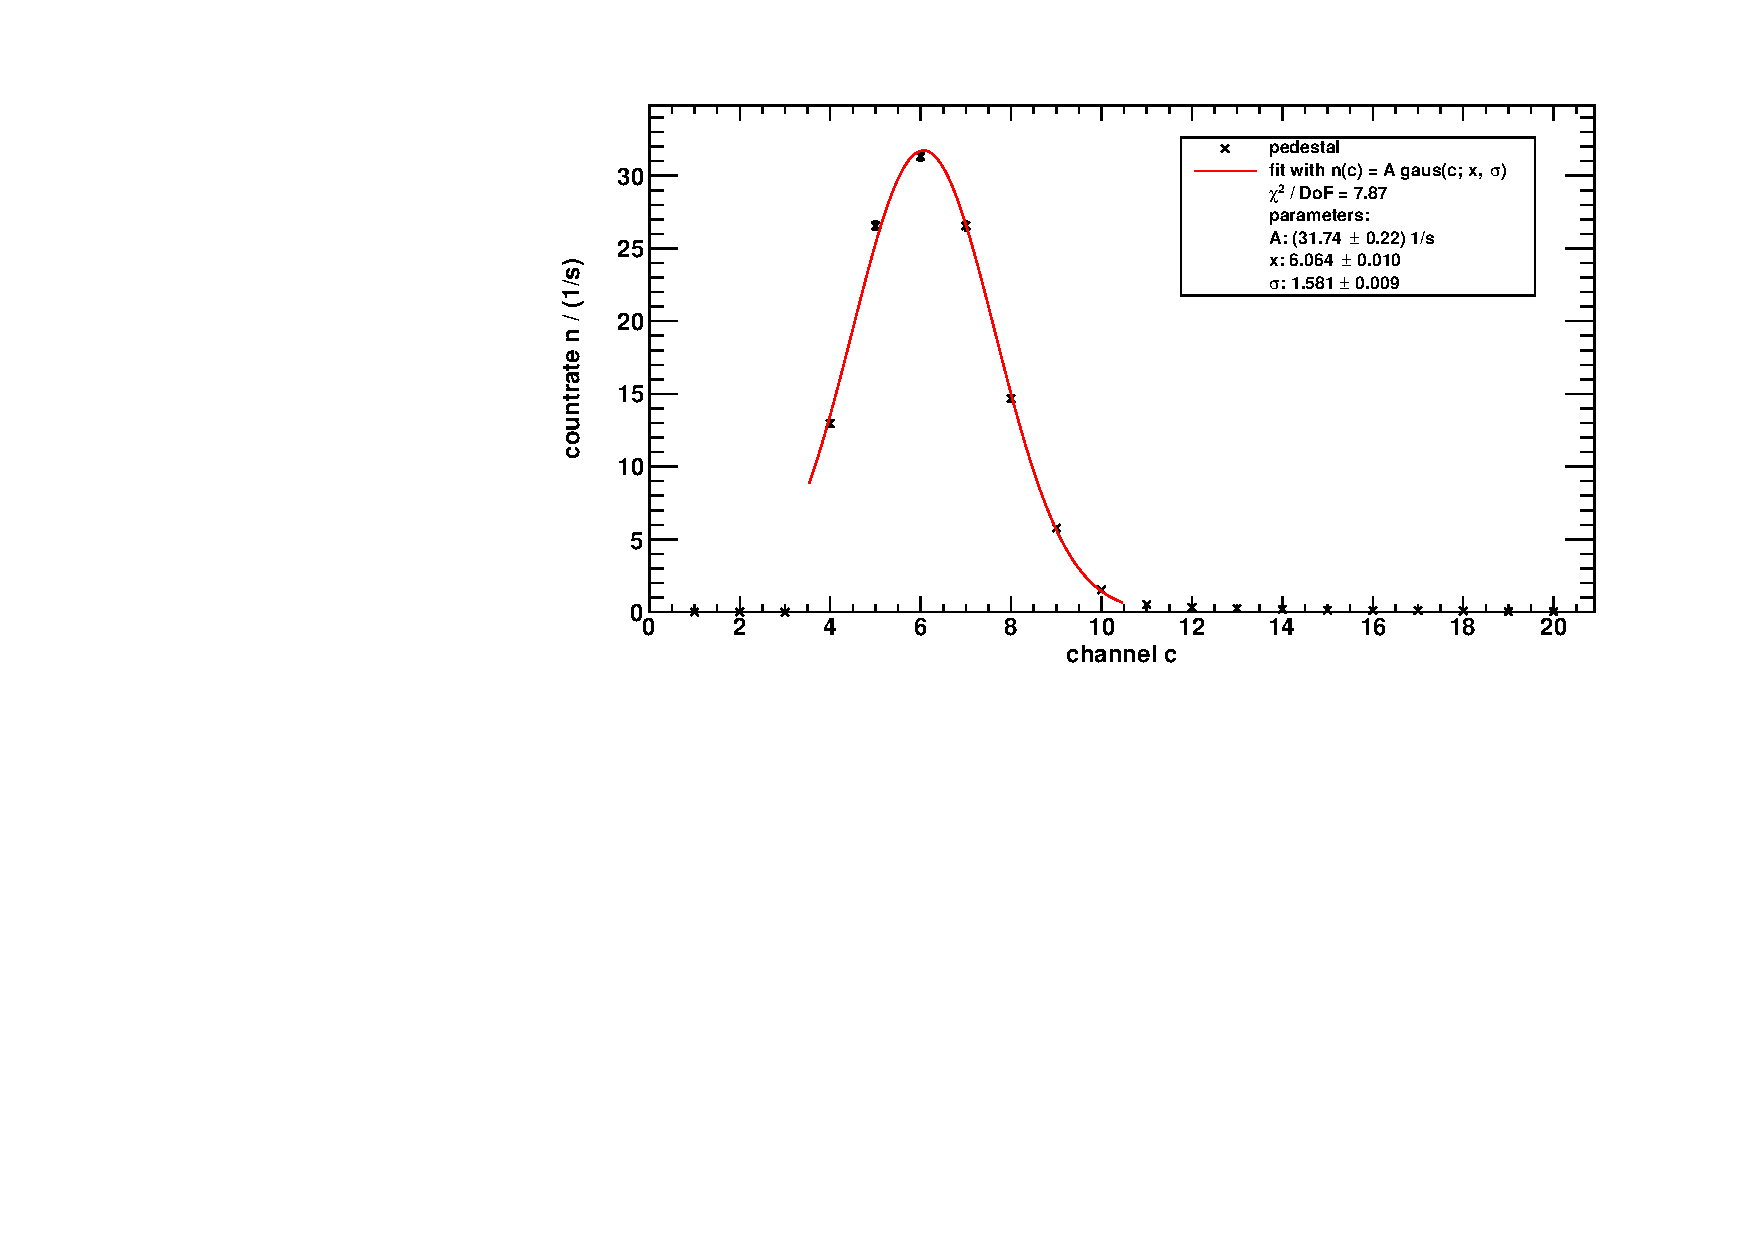
\includegraphics[width=\textwidth]{../img/pedestal.pdf}
  \caption{Pedestal: Peak at the low end of the energy spectrum caused by opening the linear gate without the occurrence of a passing signal. 
  The reason for the pedestal is shown in \autoref{img:delcapgate}.}
  \label{img:pedestal}
\end{center}
\end{figure}
The peak is fitted with the Gaussian distribution multiplied by an amplitude $A$:
\begin{equation}
    n(c) = A \cdot \gaus(c;x,\sigma)
\end{equation}
The expectation value of the fitted Gaussian distribution is:
\begin{equation}
    x = (6.064 \pm 0.010)
\end{equation}

\subsubsection{Flight through spectra}
\label{subsub:flightthroughspectra}
\paragraph{Landau distribution}
The Landau distribution describes the fluctuations of energy loss caused by impact 
ionization\footnote{The distribution follows from the \emph{Bethe formula}.}.
But the measured data is not described by just a Landau distribution, since the spectrum is blurred by the energy resolution of the scintillator. 
To get a function for fitting a convolution of the Landau distribution with a Gaussian distribution is needed:
\begin{equation}
    \label{eq:landaugausconv}
    (\landau(\mu, s) *  \gaus(0, \sigma))(c) = \int_{-\infty}^{\infty} \landau(x;\mu, s) \gaus(c-x;0,\sigma)\difd x
\end{equation}
Since there is no analytical closed form for the Landau distribution the convolution can not be solved analytical. The spectra are fitted with a
numerical convolution\footnote{The code is based on \url{https://root.cern.ch/root/html/tutorials/fit/langaus.C.html}, translated to Python by us.}. 
The spectra with their fits are shown in \autoref{img:ecal:100}, \autoref{img:ecal:50} and \autoref{img:ecal:35}. The fitted parameters are listed in 
\autoref{tab:ecal}.
\begin{figure}[H]
\begin{center}
  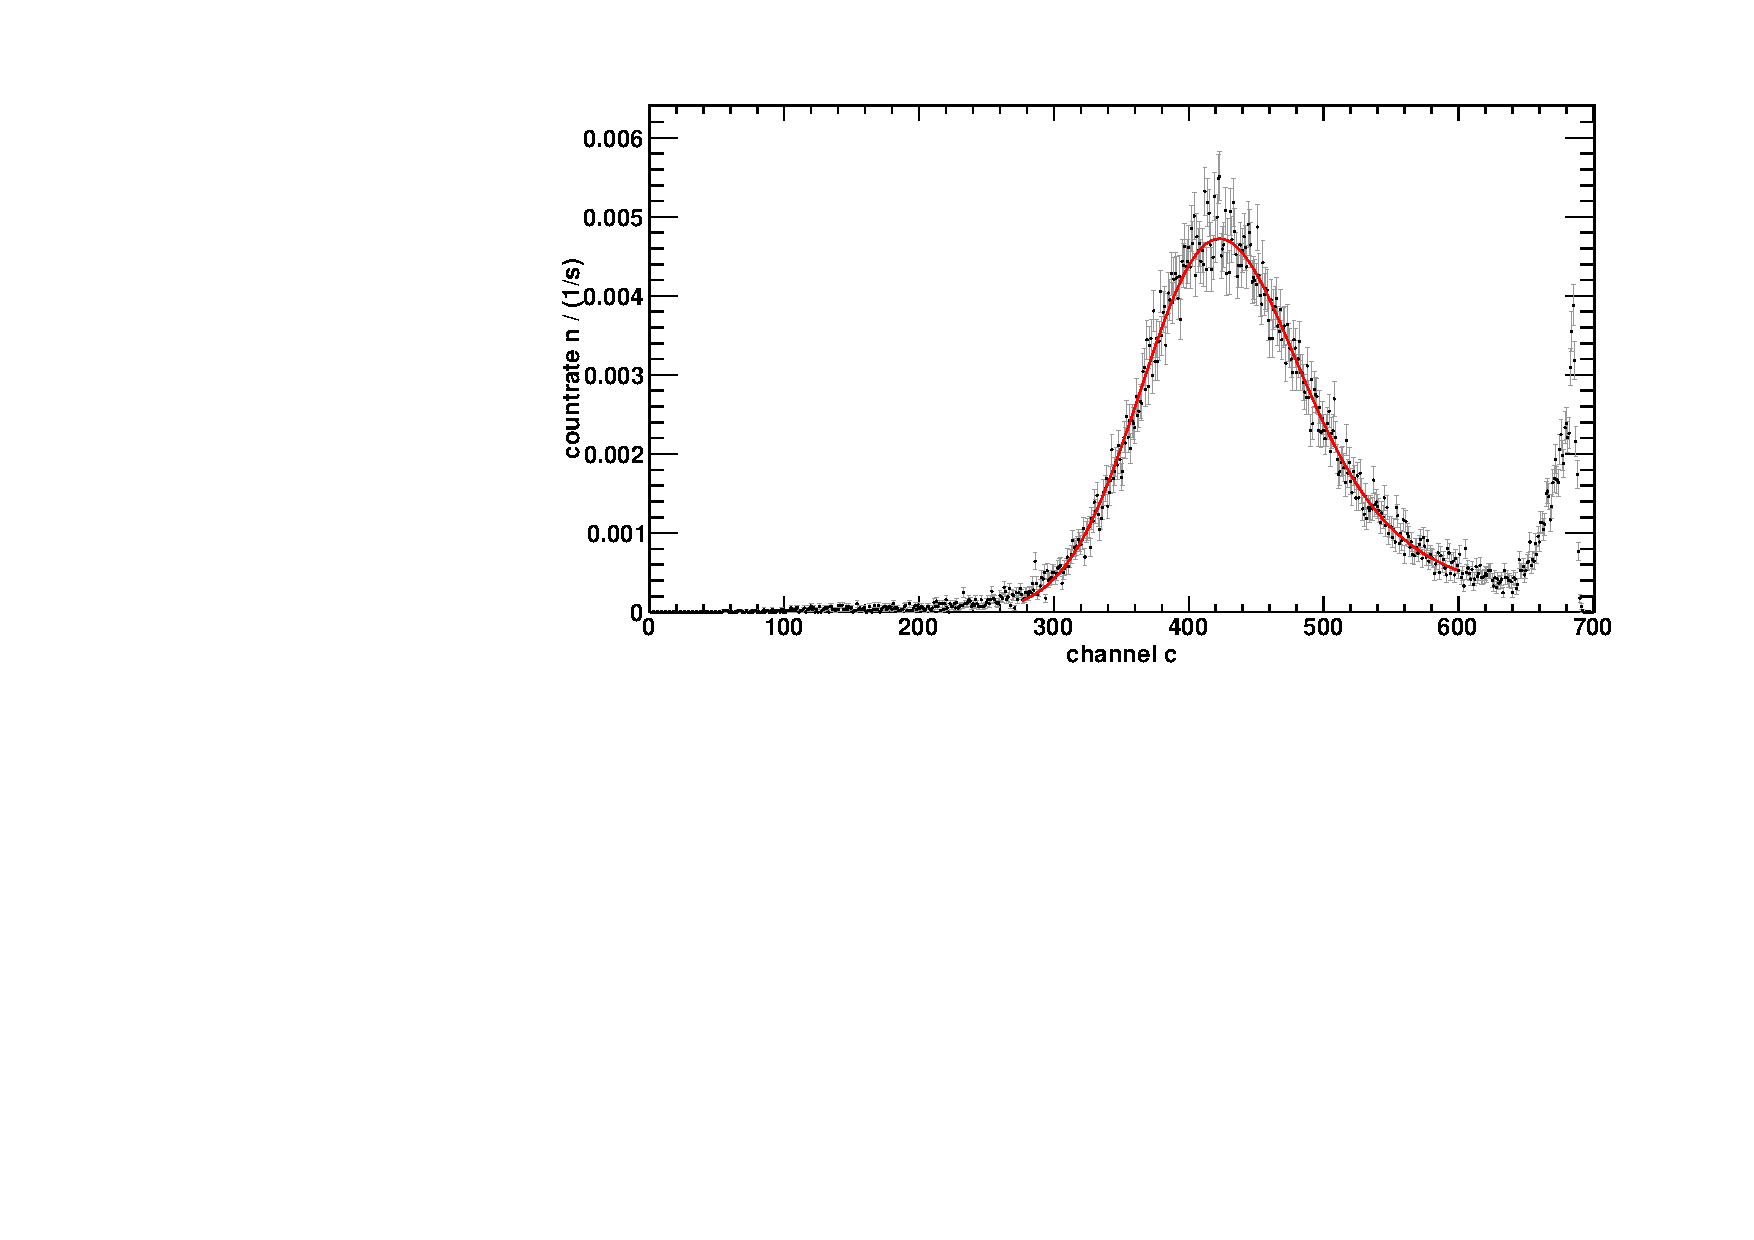
\includegraphics[width=\textwidth]{../img/energiekalibration_100.pdf}
  \caption{Flight through spectrum of muons with 12\,dB attenuation ($\overset{\wedge}{=}$ 100\% energy) with a blurred Landau fit.}
  \label{img:ecal:100}
\end{center}
\end{figure}

\begin{figure}[H]
\begin{center}
  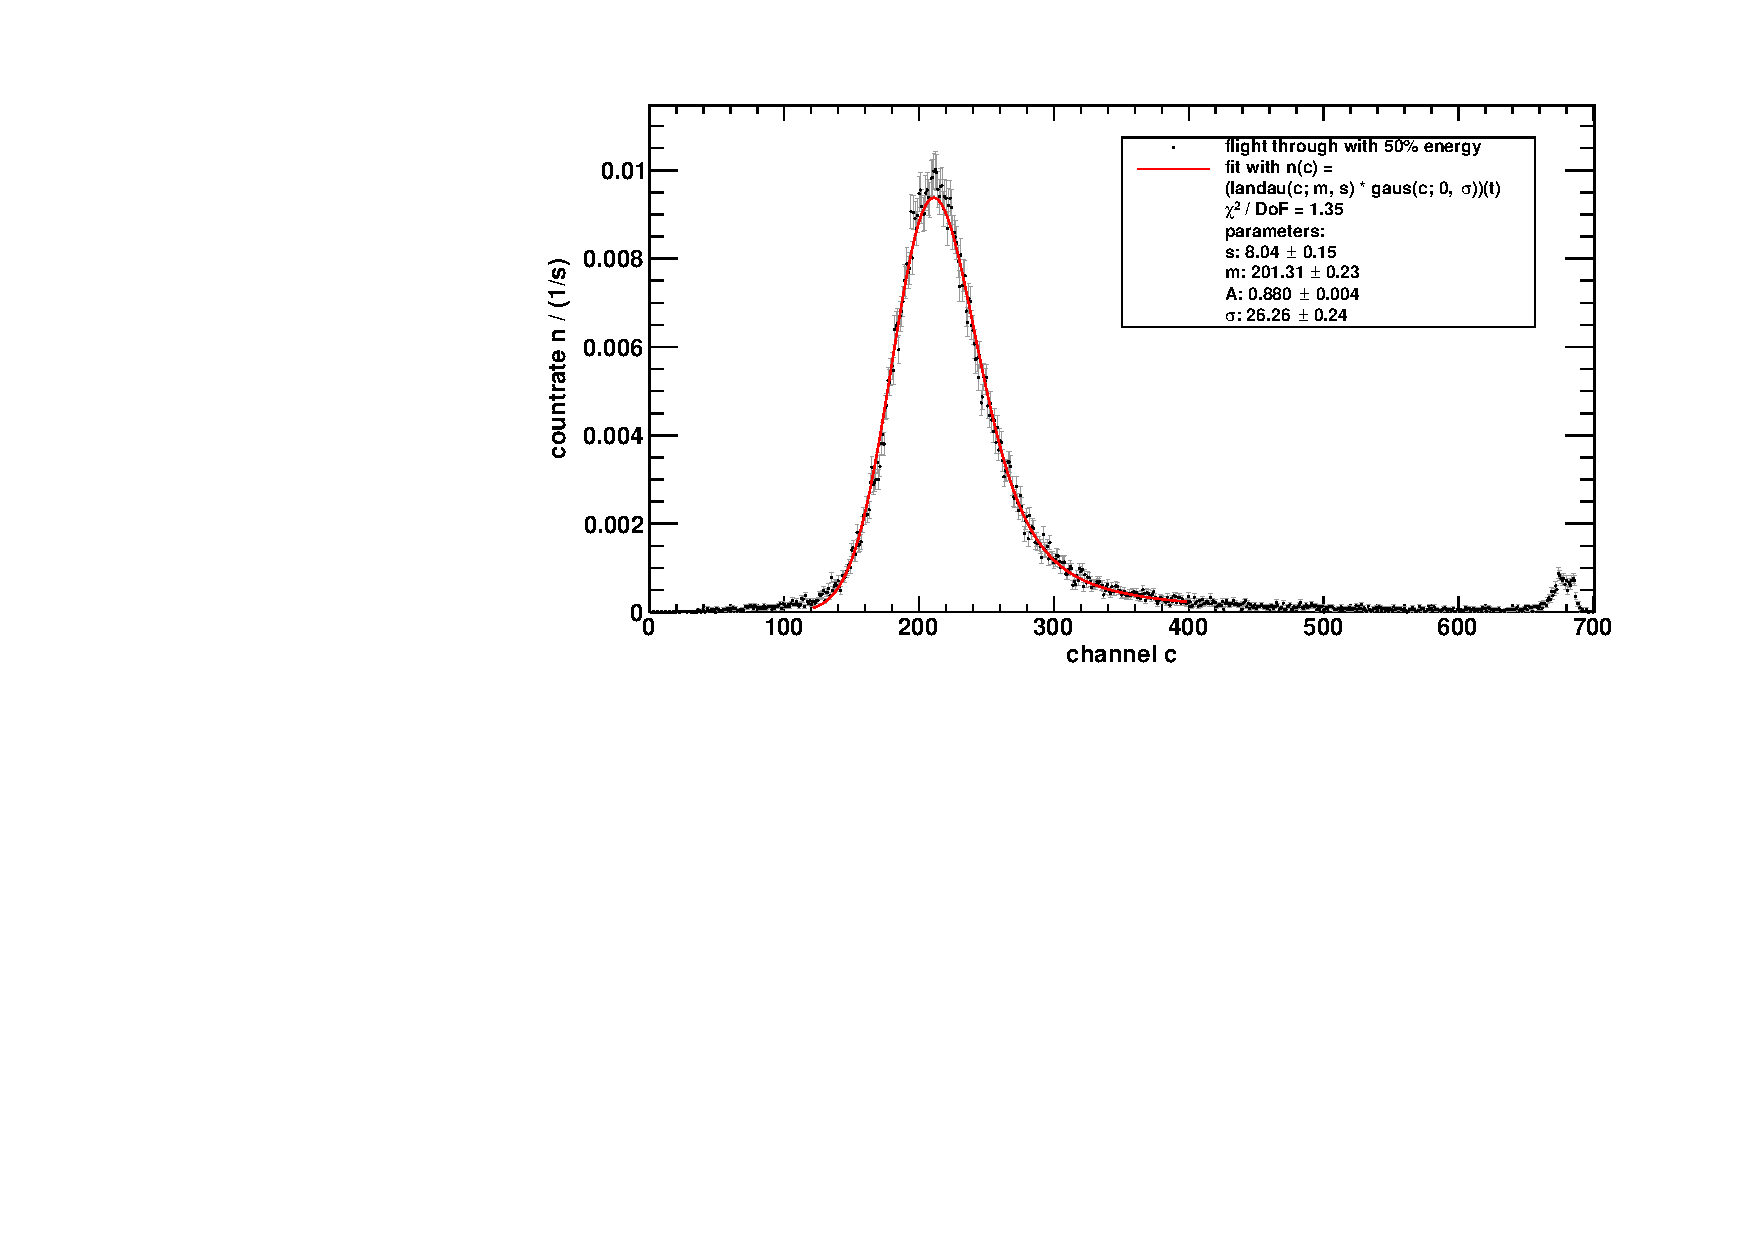
\includegraphics[width=\textwidth]{../img/energiekalibration_50.pdf}
  \caption{Flight through spectrum of muons with 18\,dB attenuation ($\overset{\wedge}{=}$ 50\% energy) with a blurred Landau fit.}
  \label{img:ecal:50}
\end{center}
\end{figure}

\begin{figure}[H]
\begin{center}
  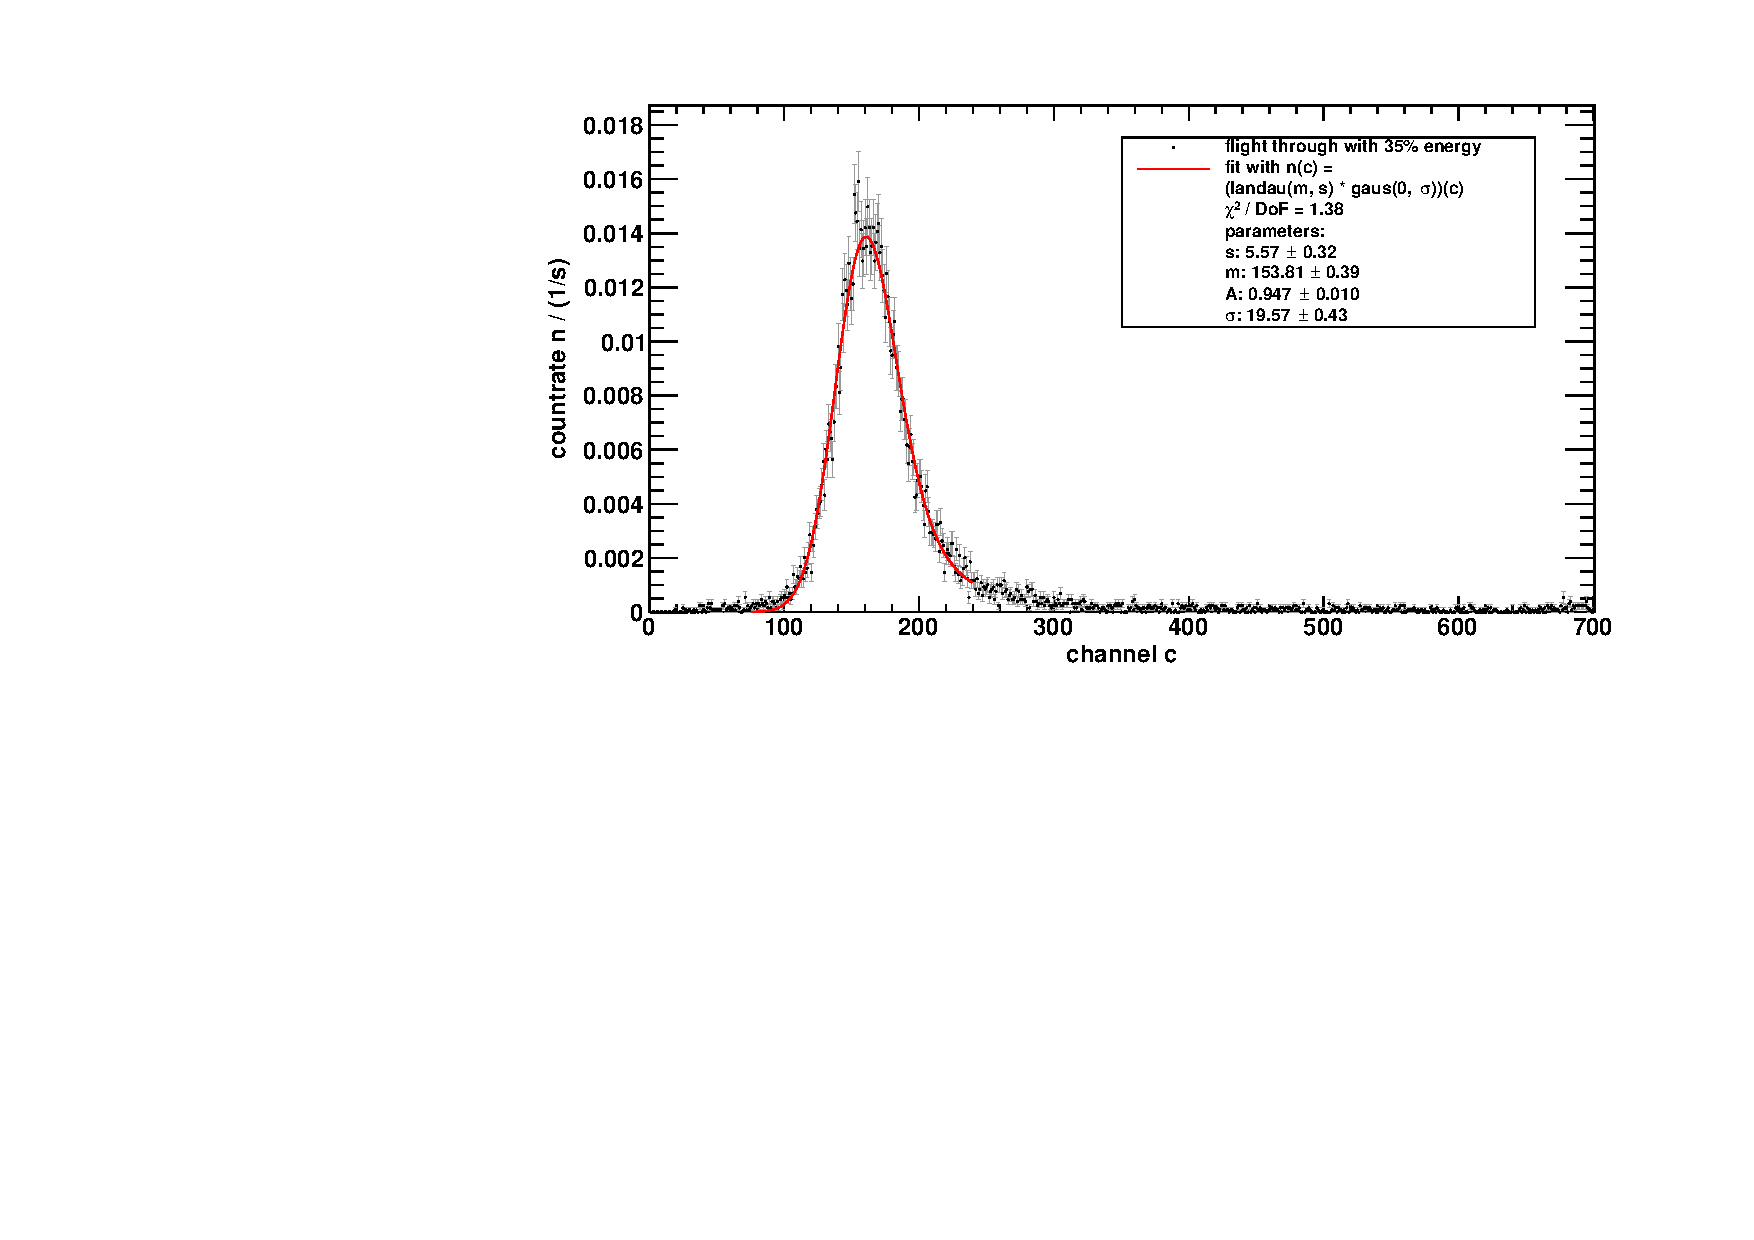
\includegraphics[width=\textwidth]{../img/energiekalibration_35.pdf}
  \caption{Flight through spectrum of muons with 21\,dB attenuation ($\overset{\wedge}{=}$ 35\% energy) with a blurred Landau fit.}
  \label{img:ecal:35}
\end{center}
\end{figure}

\subsubsection{Verification of the attenuator}
The measured amplitudes $A$ of the attenuated signals are shown in \autoref{tab:attenuator}.
\begin{table}[H]
\caption{Measured amplitude $A$ of a periodic rectangular signal after the attenuation with nominal value $n$.}
\begin{center}
\begin{tabular}{|c|c|c|}
    \hline
    $n$ / dB 	& $A$ / mV 	& $s_A$ / mV	\\ \hline \hline
    0 			& 840		& 40			\\ \hline
    12			& 210		& 10			\\ \hline
    18			& 106		& 4				\\ \hline
    21			& 75		& 4				\\ \hline
\end{tabular}
\end{center}
\label{tab:attenuator}
\end{table}
The measured attenuation $m$ can be calculated with
\begin{equation}
    m = - 20 \log_{10} \left( \frac{A}{A_0} \right), \qquad s_m = \frac{20}{\ln 10} \sqrt{ \left( \frac{s_A}{A} \right)^2 + \left( \frac{s_{A_0}}{A_0} \right)^2}
\end{equation}
where $A_0$ is the the amplitude at $n=0$\,dB.
Those attenuations can be plotted against the nominal values (\autoref{img:attenuator}).
\begin{figure}[H]
\begin{center}
  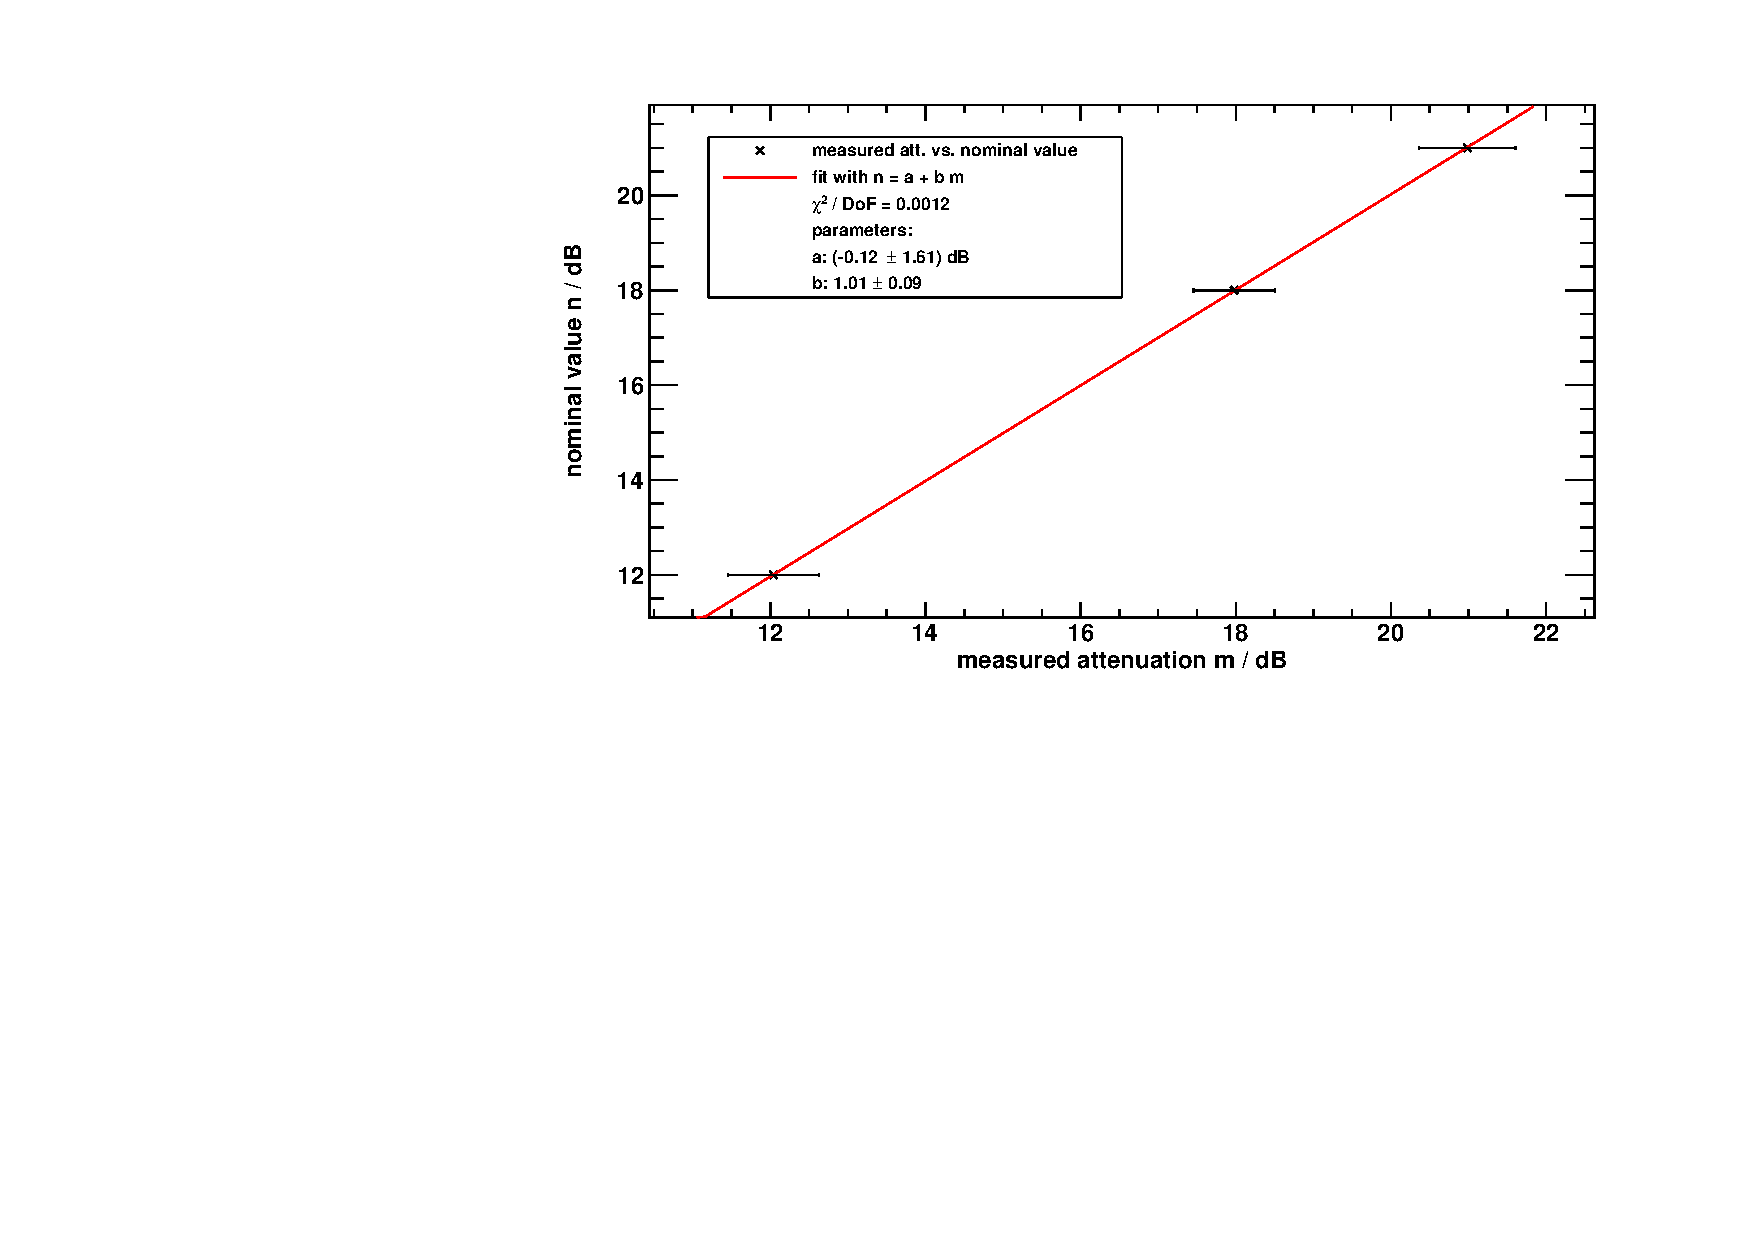
\includegraphics[width=\textwidth]{../img/attenuator.pdf}
  \caption{Nominal attenuations $n$ plotted against the measured attenuations $m$ and fit with a line.}
  \label{img:attenuator}
\end{center}
\end{figure}
If the attenuator works correctly, the linear fit should yield a line with intercept $a=0$\,dB and slope $b=1$. The fit results are:
\begin{equation}
    \begin{split}
        & a = (-0.1 \pm 1.6)\,\text{dB} \\
        & b = 1.01  \pm 0.09 
    \end{split}
\end{equation}
Therefore we conclude that the attenuator works correctly and no correction is needed.

\subsubsection{Calibration}
For the calibration it must be known how much energy a muon deposits in the tank. Following data was given:
\begin{equation}
    \begin{split}
        & \frac{\partial E}{\partial \rho x} = (1.95 \pm 0.05)\,\frac{\text{MeV}\cdot\text{cm}^2}{\text{g}} \qquad \text{(minimal ionizing muon)}  \\
        & \rho = (0.87 \pm 0.01) \, \frac{\text{g}}{\text{cm}^3}  \qquad \qquad \qquad \text{(density of solvent)} \\
        & s = (84 \pm 5) \, \text{cm} \qquad \qquad \qquad \qquad \quad  \text{(mean free path in tank)}
    \end{split}
\end{equation}
Hence the total loss of energy calculates to:
\begin{equation}
    \begin{split}
        & E = \frac{\partial E}{\partial \rho x} \cdot \rho \cdot s = 142.5\,\text{MeV} \\
        & s_{E} = E \cdot \sqrt{ \left( \frac{s_{\frac{\partial E}{\partial \rho x}}}{\frac{\partial E}{\partial \rho x}} \right)^2 + \left( \frac{s_\rho}{\rho} \right)^2 + \left( \frac{s_s}{s} \right)^2  }
        = 9.4
    \end{split}
\end{equation}
The percentage loss of energy can now be determined:
\begin{equation}
    E_p = p \cdot E, \qquad s_{E_p} = p \cdot s_E, \qquad 0 \leq p \leq 1  %TODO Fehler auf p wegen Dämpfer?
\end{equation}
The fitted peaks of the energy calibration and their respective energies are listed in \autoref{tab:ecal} and visualized in \autoref{img:energycalibration}.
\begin{table}[H]
\caption{Channels of fitted peaks and their theoretical energy for the energy calibration.}
\begin{center}
\begin{tabular}{|c|c|c|c|c|}
  \hline
  \% energy & $c$ & $s_c$ & $E$ / MeV & $s_E$ / MeV \\ \hline
  0 & 6.064 & 0.010 & 0.0 & 0.0 \\ \hline
  35 & 153.808 & 0.392 & 49.9 & 3.0 \\ \hline
  50 & 201.312 & 0.225 & 71.3 & 4.3 \\ \hline
  100 & 404.770 & 0.547 & 142.5 & 8.5 \\ \hline
\end{tabular}
\end{center}
\label{tab:ecal}
\end{table}

\begin{figure}[H]
\begin{center}
  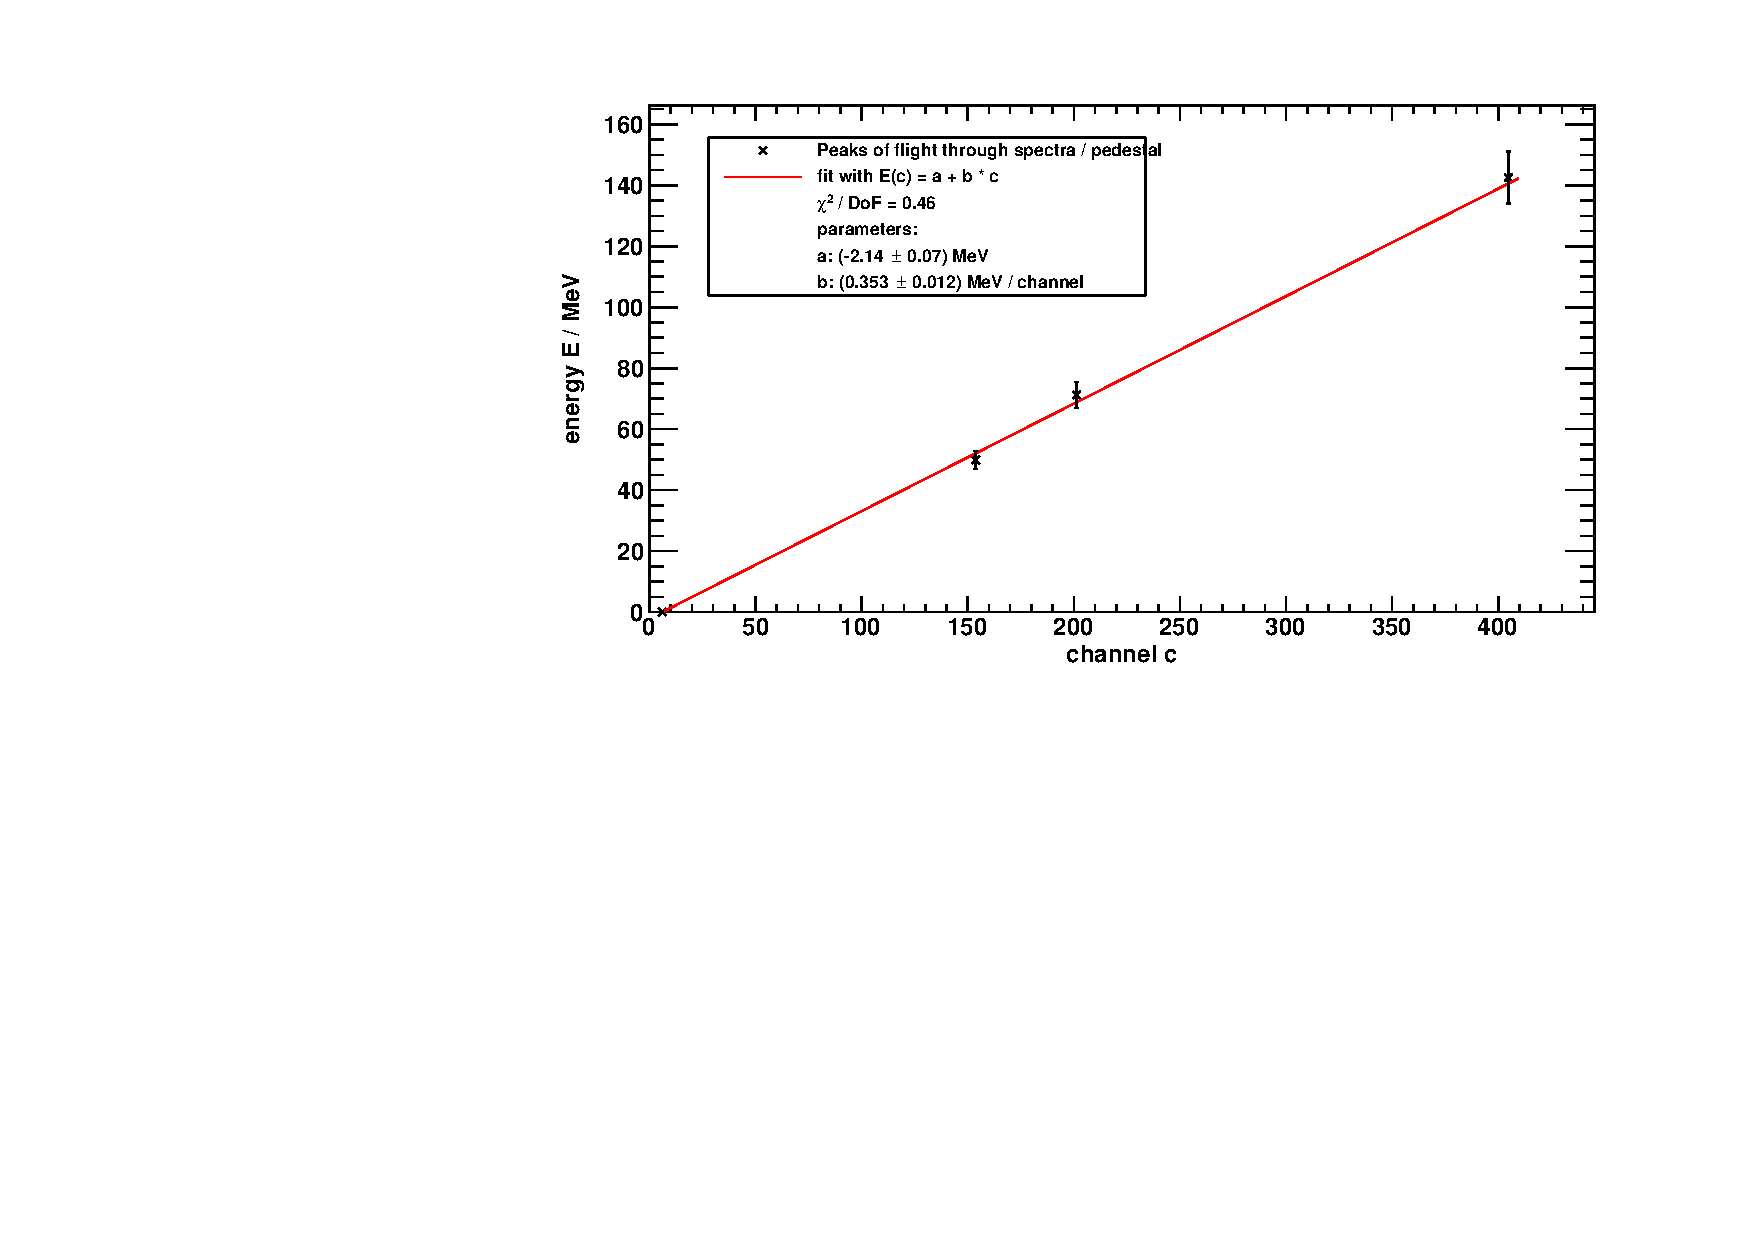
\includegraphics[width=\textwidth]{../img/energyCalibration.pdf}
  \caption{Energy calibration.}
  \label{img:energycalibration}
\end{center}
\end{figure}
Since the scintillators should produce a signal amplitude linear to the measured energy, a linear fit is implemented:
\begin{equation}
    E(c) = a + b \cdot c
\end{equation}
The fit yields:
\begin{equation}
    \begin{split}
        & a = (-2.14 \pm 0.07) \, \text{MeV} \\
        & b = (0.353 \pm 0.012) \, \frac{\text{MeV}}{\text{channel}} \\
        & \cov(a, b) = -0.0009 \, \frac{\text{MeV}^2}{\text{channel}} 
    \end{split}
\end{equation}
Now the energy $E$ of a channel $c$ and its error $s_E$ can be calculated with:
\begin{equation}
\label{eq:ecalibration}
    E = a + b \cdot c, \qquad s_E = \sqrt{s_a^2 + \left(c \cdot s_b \right)^2 + 2 \cdot c \cdot \cov(a,b)}
\end{equation}

\subsection{Time calibration}
In \autoref{tab:tcal} the data for the time calibration is listed.
In each of the four measurements, there were only one or two channels of MCA\,II responding,
so there is no need to fit the data.
\begin{table}[H]
\caption{Measured times and channels with errors for the time calibration.}
\begin{center}
\begin{tabular}{|c|c|c|c|}
  \hline
  $t$ / \textmu s & $s_t$ / \textmu s & $c$ & $s_c$ \\ \hline
  2.40 & 0.02 & 113.0 & 0.5 \\ \hline
  4.50 & 0.02 & 223.0 & 0.5 \\ \hline
  6.25 & 0.02 & 315.5 & 0.5 \\ \hline
  8.60 & 0.02 & 441.0 & 0.5 \\ \hline
\end{tabular}
\end{center}
\label{tab:tcal}
\end{table}

A linear fit is done (\autoref{img:timecalibration}):
\begin{equation}
    t = a + b \cdot c
\end{equation}
\begin{figure}[H]
\begin{center}
  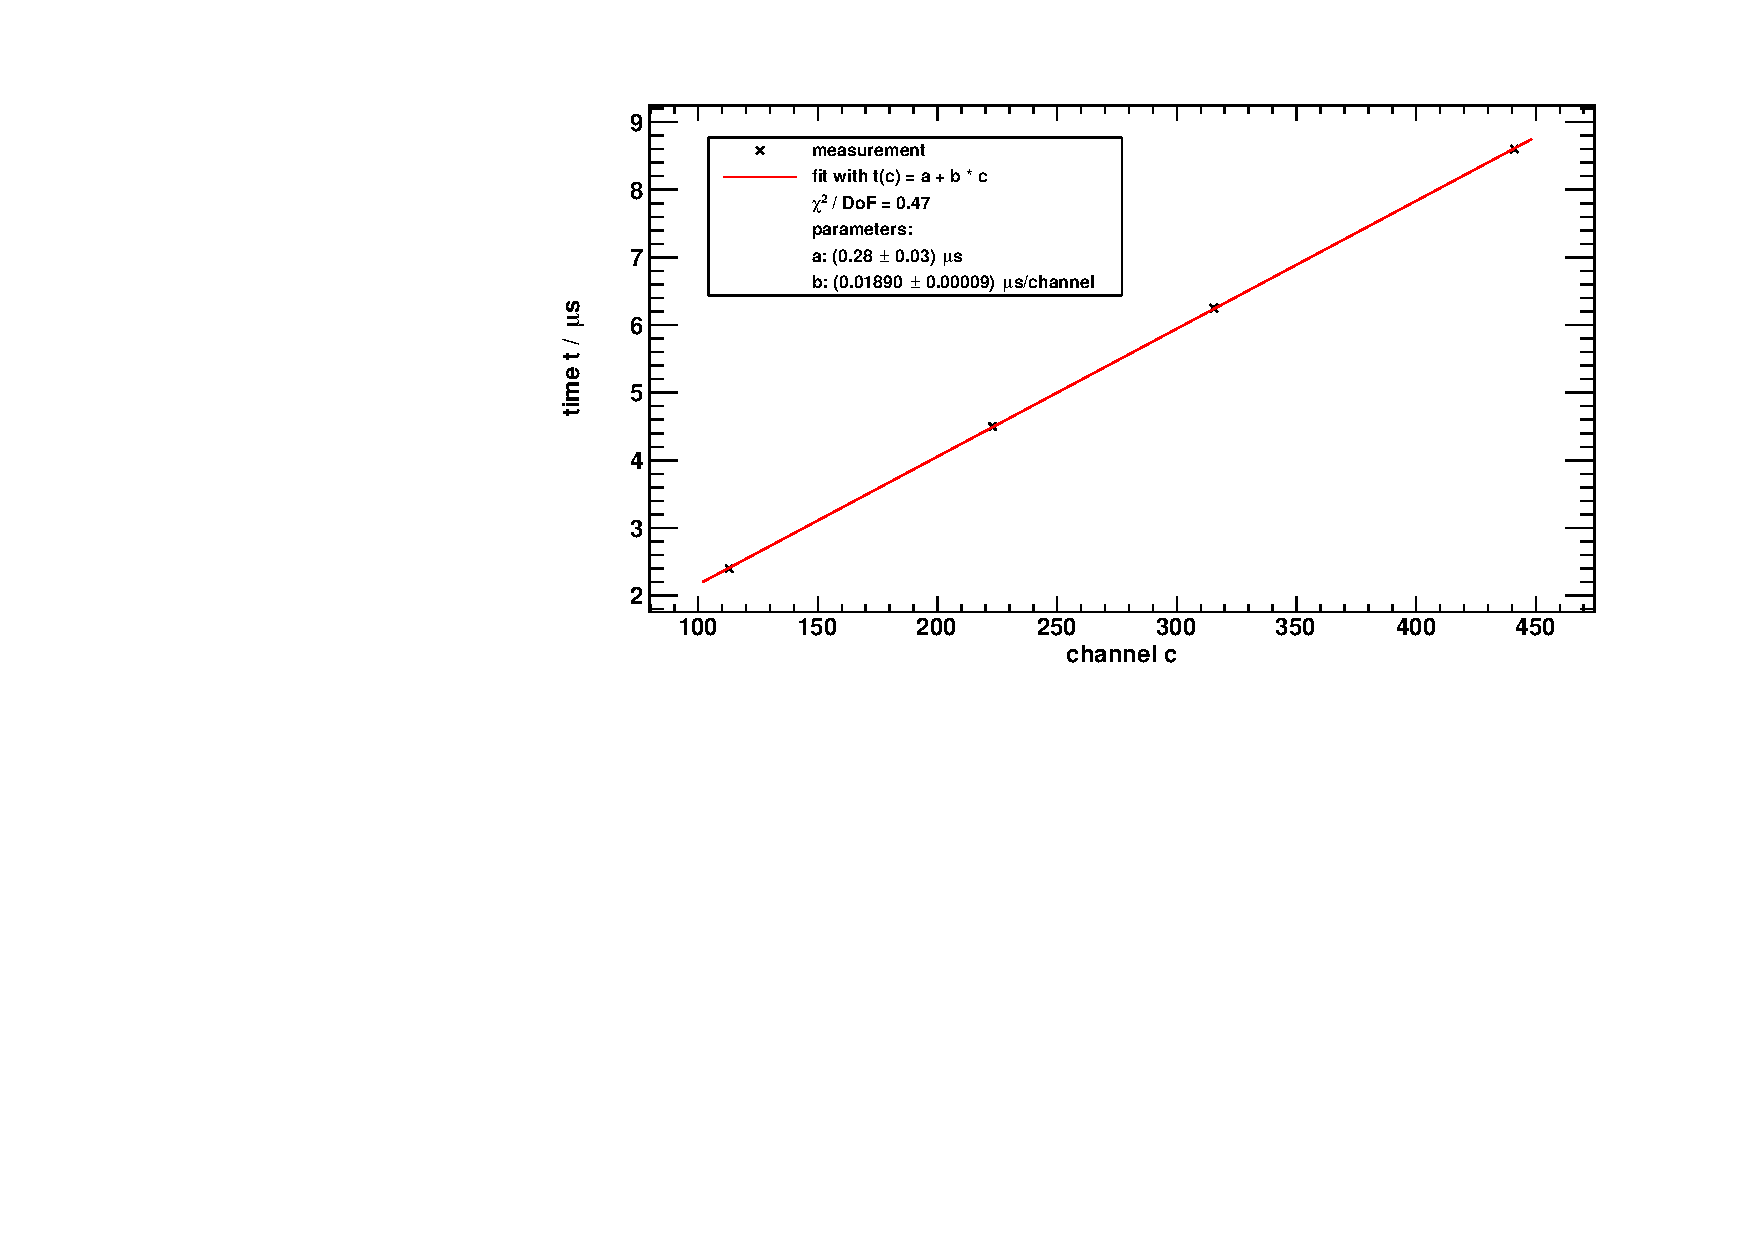
\includegraphics[width=\textwidth]{../img/timeCalibration.pdf}
  \caption{Time Calibration.}
  \label{img:timecalibration}
\end{center}
\end{figure}
The parameters and their covariance for this fit are:
\begin{equation}
    \begin{split}
        & a = (0.28 \pm 0.03) \, \text{\textmu s} \\
        & b = (0.01890 \pm 0.00009) \, \frac{\text{\textmu s}}{\text{channel}} \\
        & \cov(a, b) = -2.299 \, \frac{\text{\textmu s}^2}{\text{channel}} 
    \end{split}
\end{equation}
Now the time $t$ of a channel $c$ and its error $s_t$ can be calculated with:
\begin{equation}
\label{eq:tcalibration}
    t = a + b \cdot c, \qquad s_t = \sqrt{s_a^2 + \left(t \cdot s_b \right)^2 + 2 \cdot t \cdot \cov(a,b)}
\end{equation}

\subsection{Underground}
The underground measurement is visualized in \autoref{img:underground}.
\begin{figure}[H]
\begin{center}
  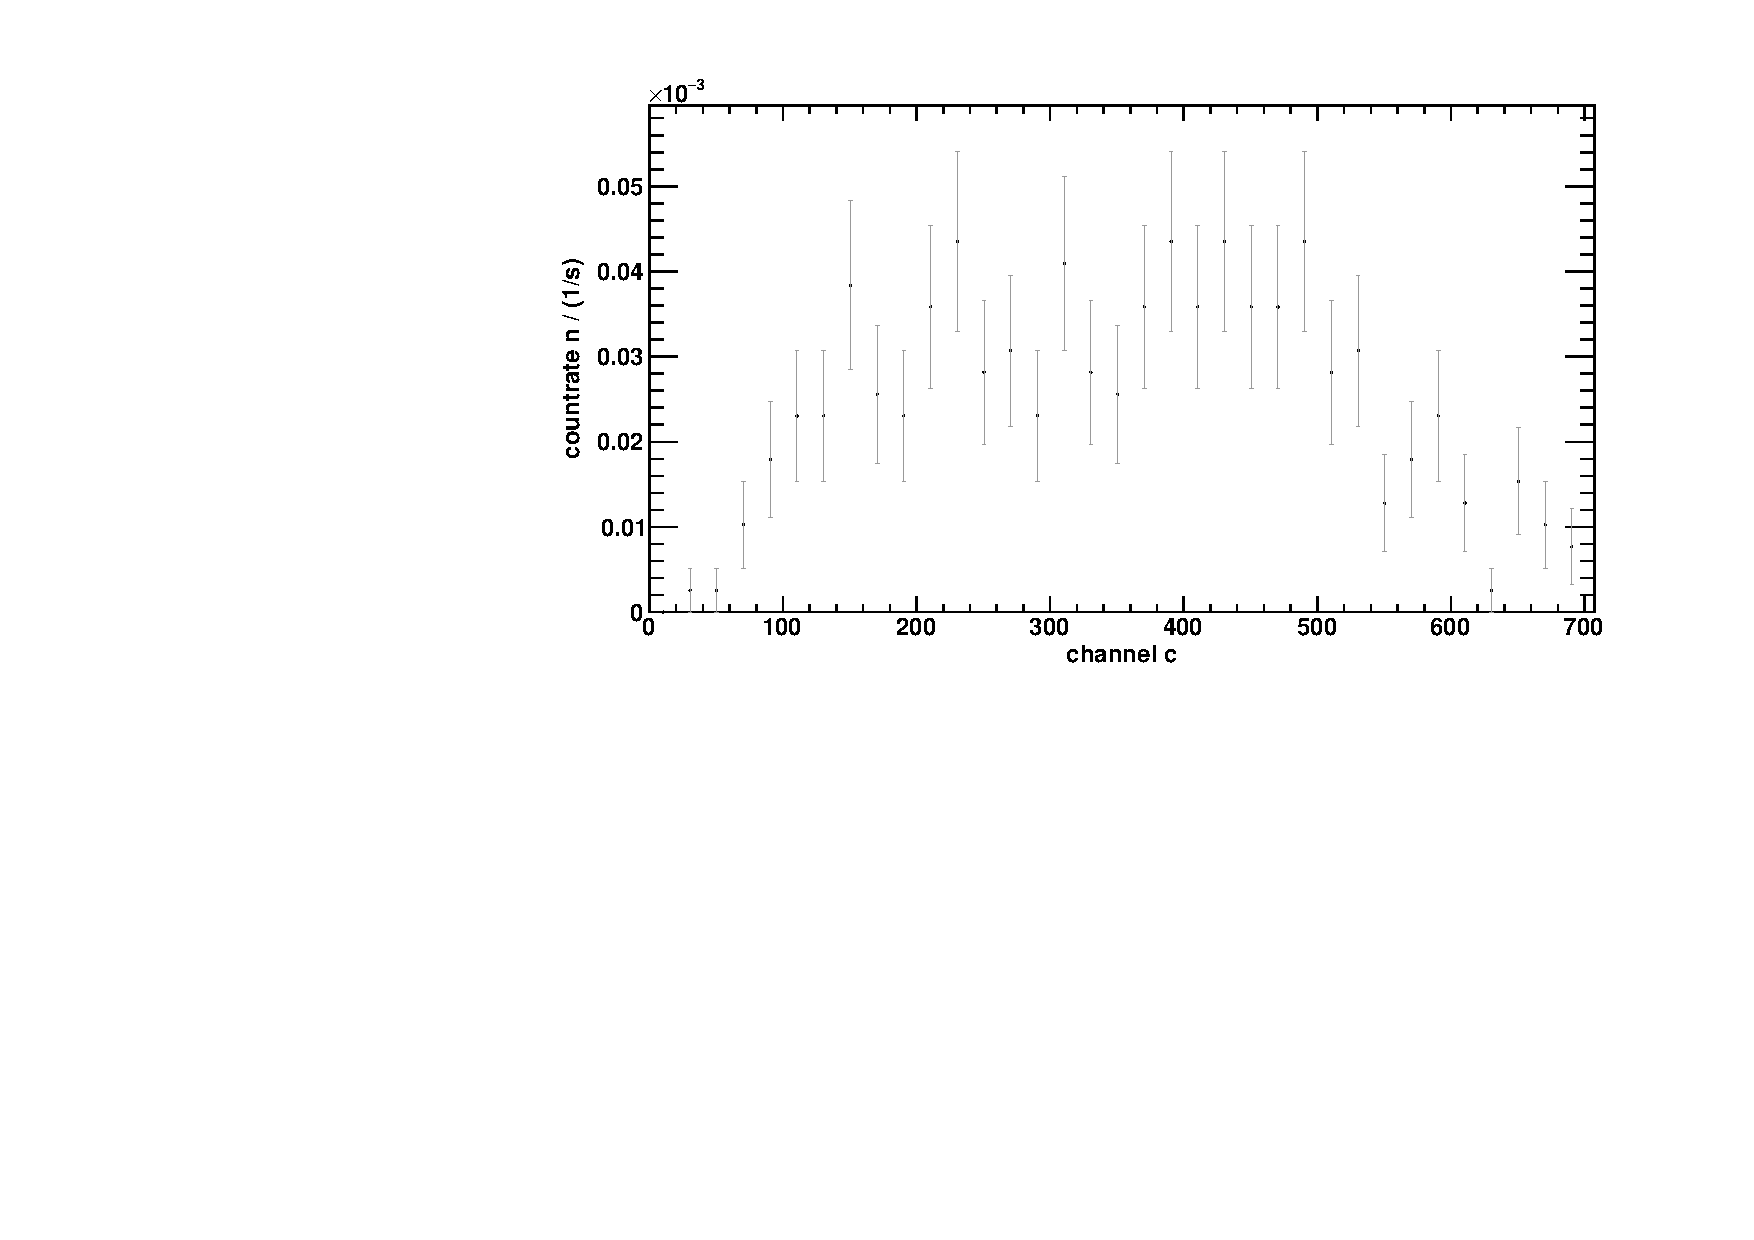
\includegraphics[width=\textwidth]{../img/underground.pdf}
  \caption{Underground.}
  \label{img:underground}
\end{center}
\end{figure}

\begin{figure}[H]
\begin{center}
  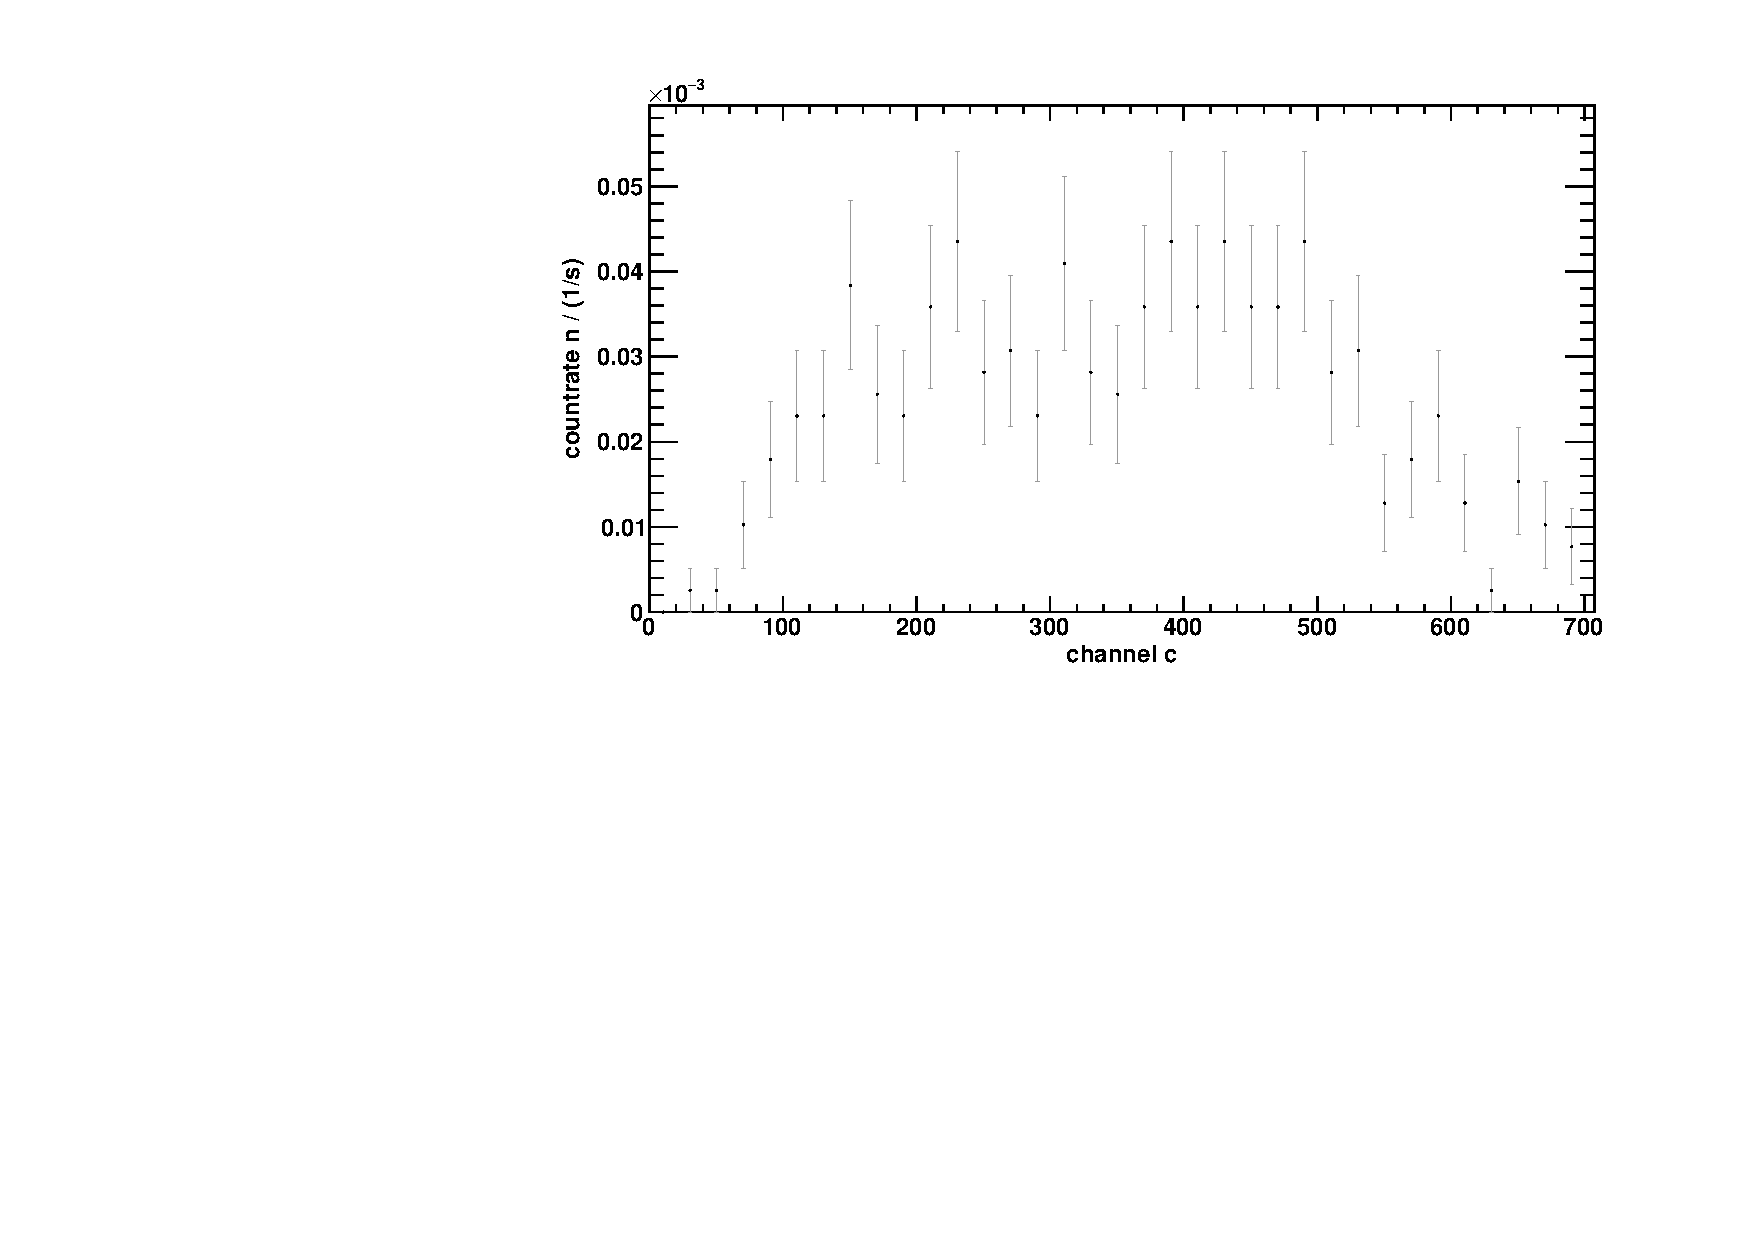
\includegraphics[width=\textwidth]{../img/underground_rebin.pdf}
  \caption{Rebinned unerground.}
  \label{img:underground:rebin}
\end{center}
\end{figure}

\subsection{\textbeta-spectrum}
The measured \textbeta-spectrum is shown in \autoref{img:beta:spectrum}.
\begin{figure}[H]
\begin{center}
  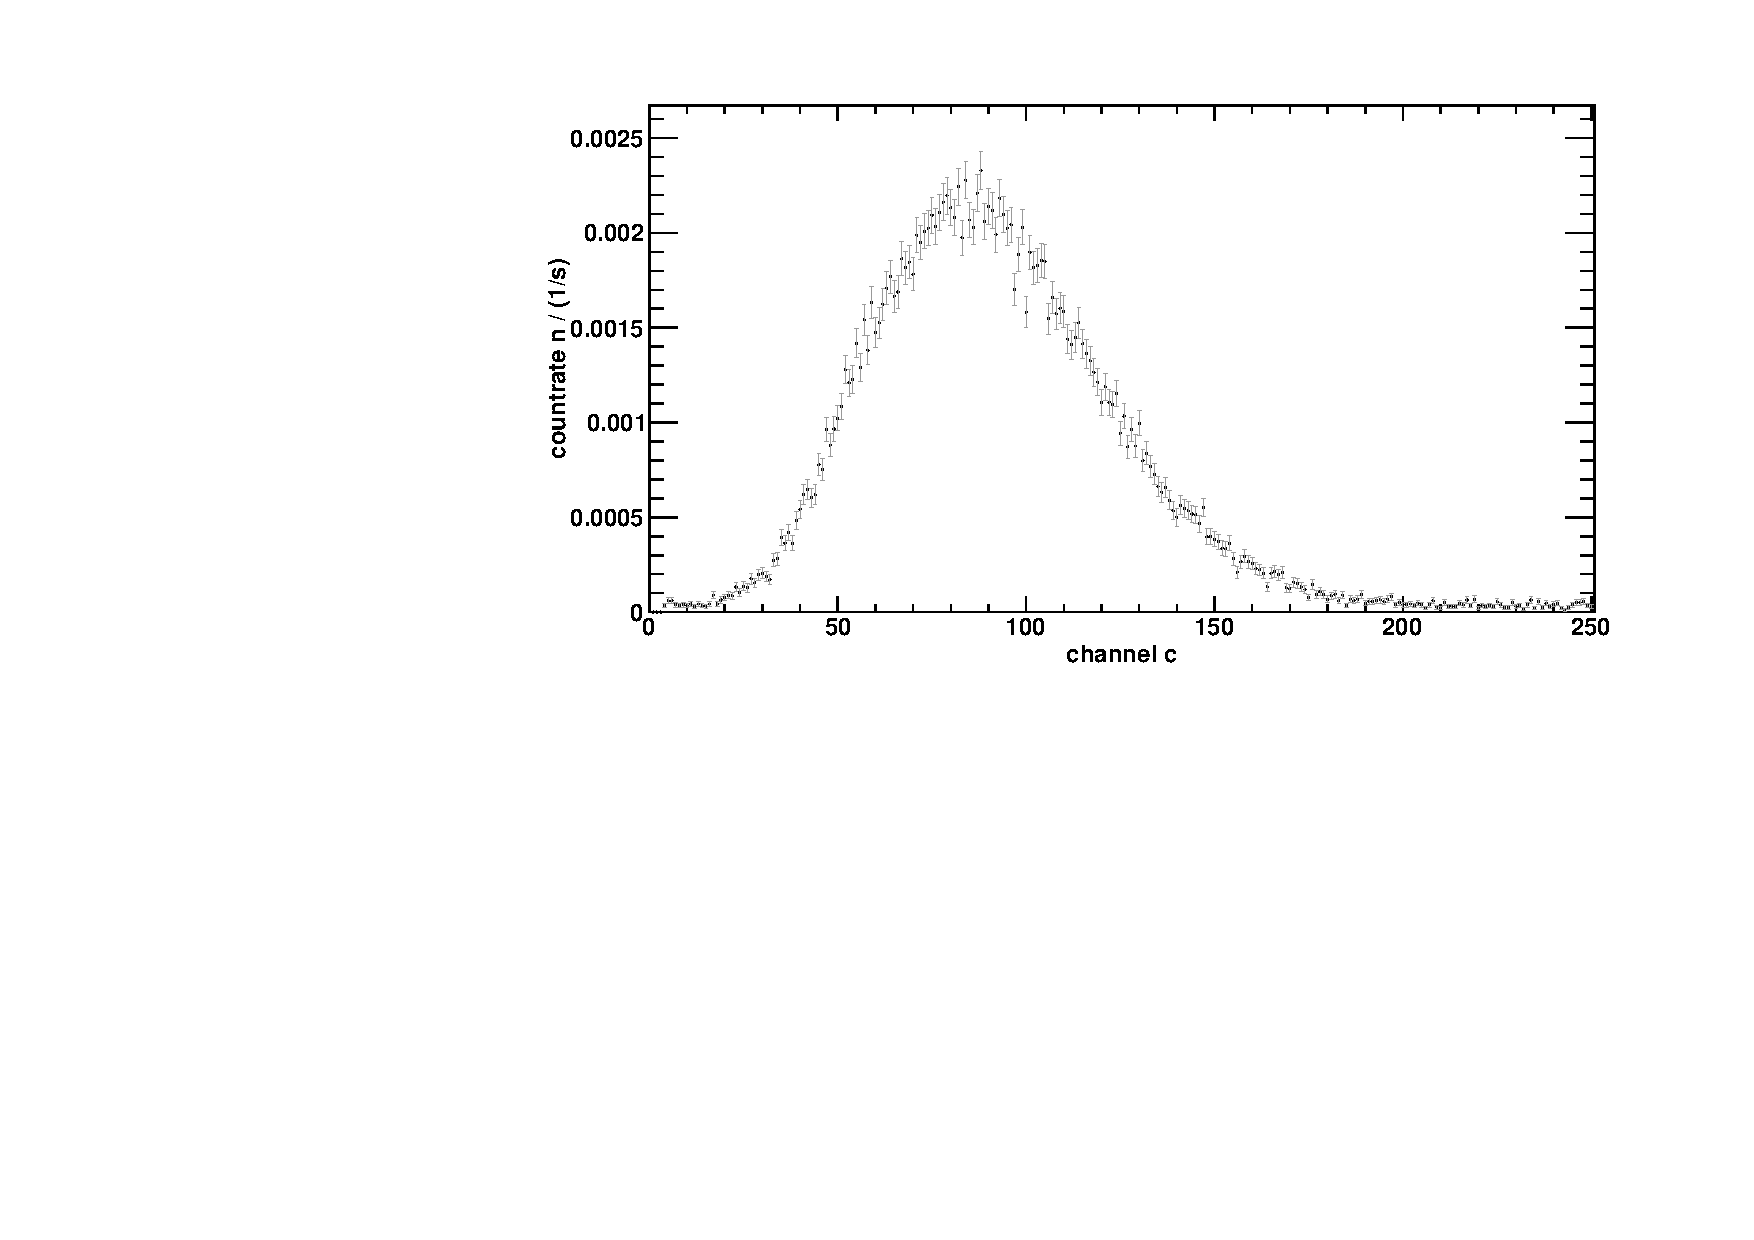
\includegraphics[width=\textwidth]{../img/betaspectrum.pdf}
  \caption{\textbeta-spectrum.}
  \label{img:beta:spectrum}
\end{center}
\end{figure}
The problem is to extract the maximal energy while taking the Gaussion blur caused by the energy resolution into account. One method is the 
\emph{Fermi-Kurie-plot} (\cite{dem4}, p.52-53).
First the channal information is converted into an energy with \autoref{eq:ecalibration}. Then $\sqrt{n(E)/E^2}$ is plotted against 
the energy $E$ (\autoref{img:beta:fermikuriefit}). Ideally a linear relationships should be identifiable. The intersection of this line with 
the $x$-axis is the maximal energy. \\
TODO warum nur teilweise linear? \\ %TODO text
The linear part gets fitted wtih
\begin{equation}
    \sqrt{n(E)/E^2} = a(E-b),
\end{equation}
so that the intersection with the $x$-axis can be read directly.
\begin{figure}[H]
\begin{center}
  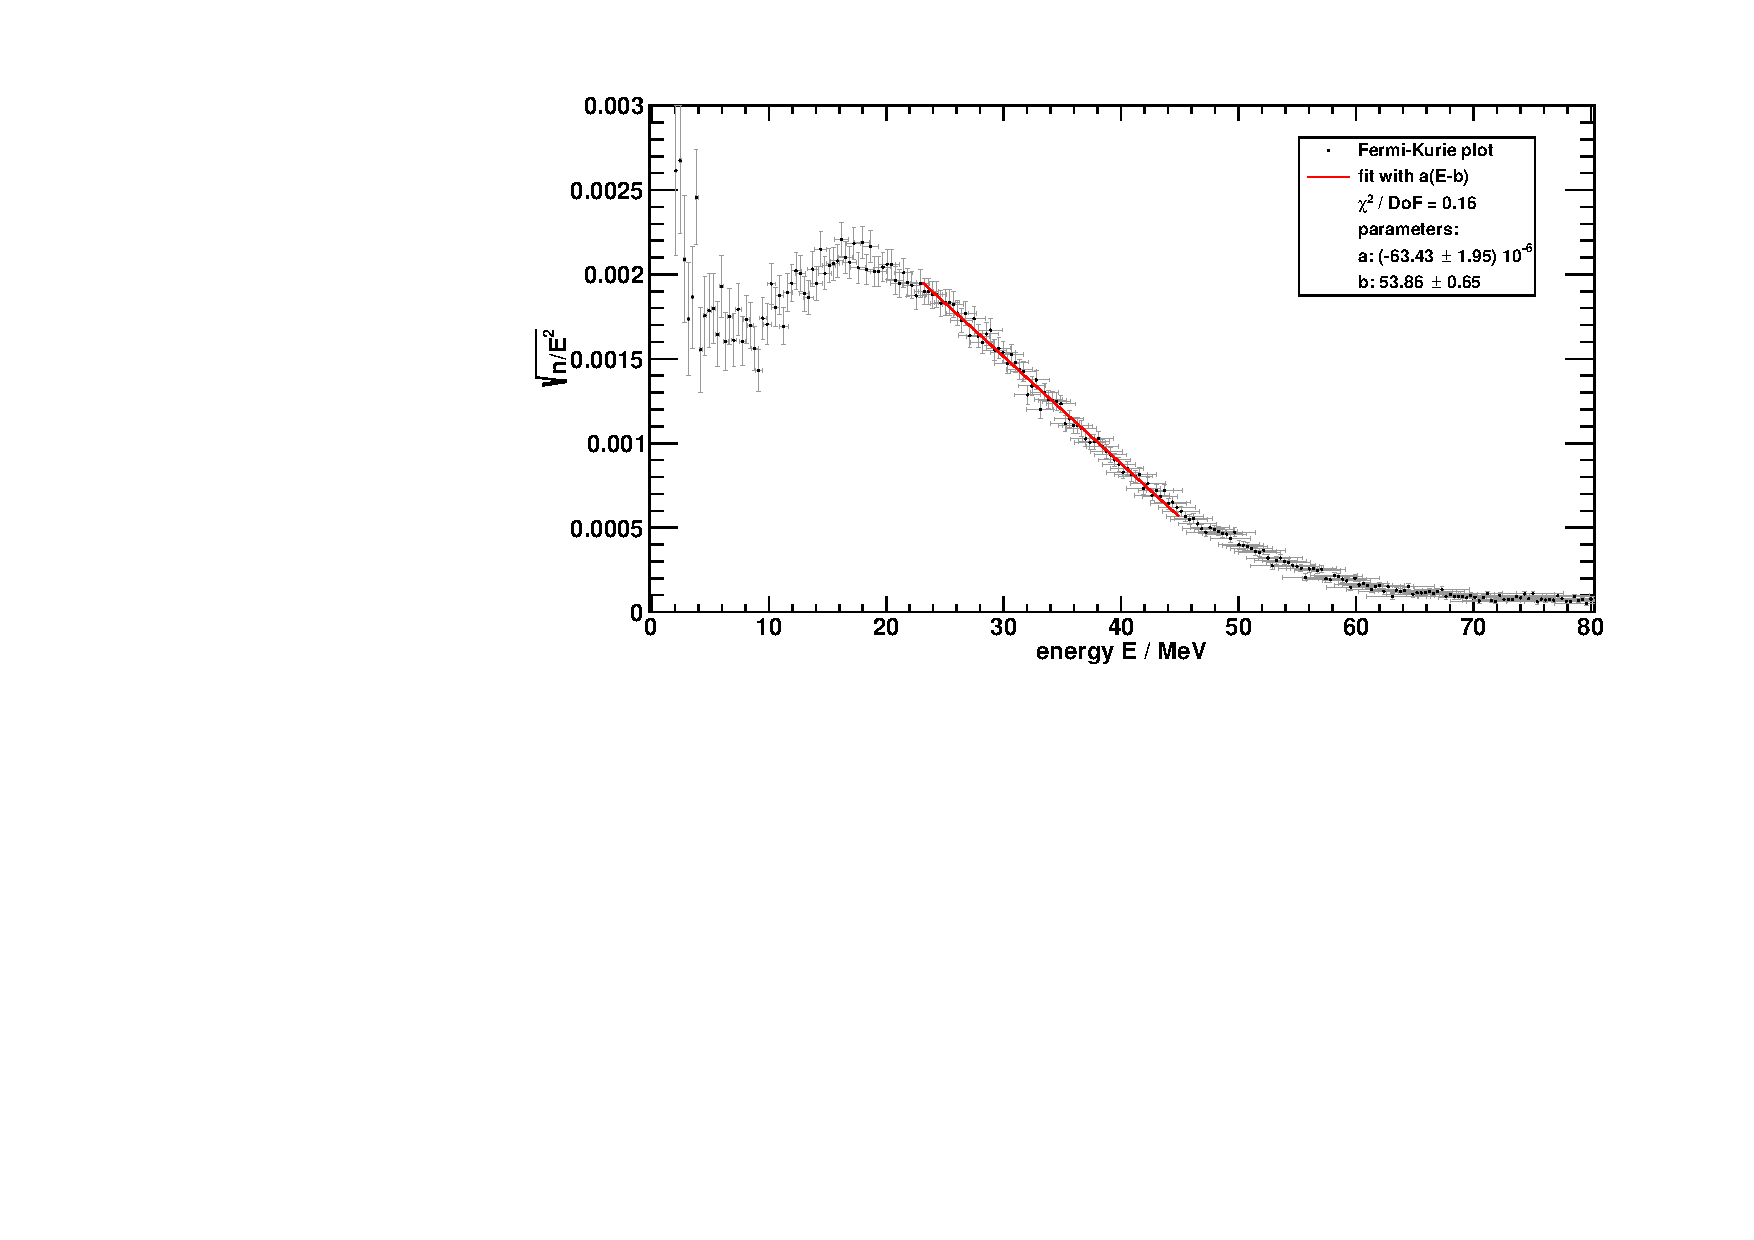
\includegraphics[width=\textwidth]{../img/betaspectrum_FermiKurie_fit.pdf}
  \caption{Fermi-Kurie plot.}
  \label{img:beta:fermikuriefit}
\end{center}
\end{figure}
With the fit one gets for $b$:
\begin{equation}
    b = (53.86 \pm 0.65)\,\text{MeV}
\end{equation}
Since this energy is half of the rest energy of the muon it has to be multiplied with 2:
\begin{equation}
\begin{split}
	\label{eq:result:mass}
    & E_\mu = 2 \cdot b, \qquad s_{E_\mu} = 2 \cdot s_b \\
    & \Rightarrow E_\mu = (107.7 \pm 1.3)\,\text{MeV}
    \end{split}
\end{equation}
The so calculated rest energy matches the literature value (\autoref{eq:litval:mass}) within a 2-\textsigma-interval.
\begin{equation}
    E_\mu^{\text{lit.}} = (105.6583715 \pm 0.0000035)\,\text{MeV}
\end{equation}

\subsection{Mean lifetime}
To calculate the mean lifetime $\tau$ of $\mu$ the channels are converted to a time with \autoref{eq:tcalibration}. 
Furthermore we rebin as described in \ref{subsub:rebinning} the spectrum to get a nicer curve. Three consecutive channels were averaged.
\begin{figure}[H]
\begin{center}
  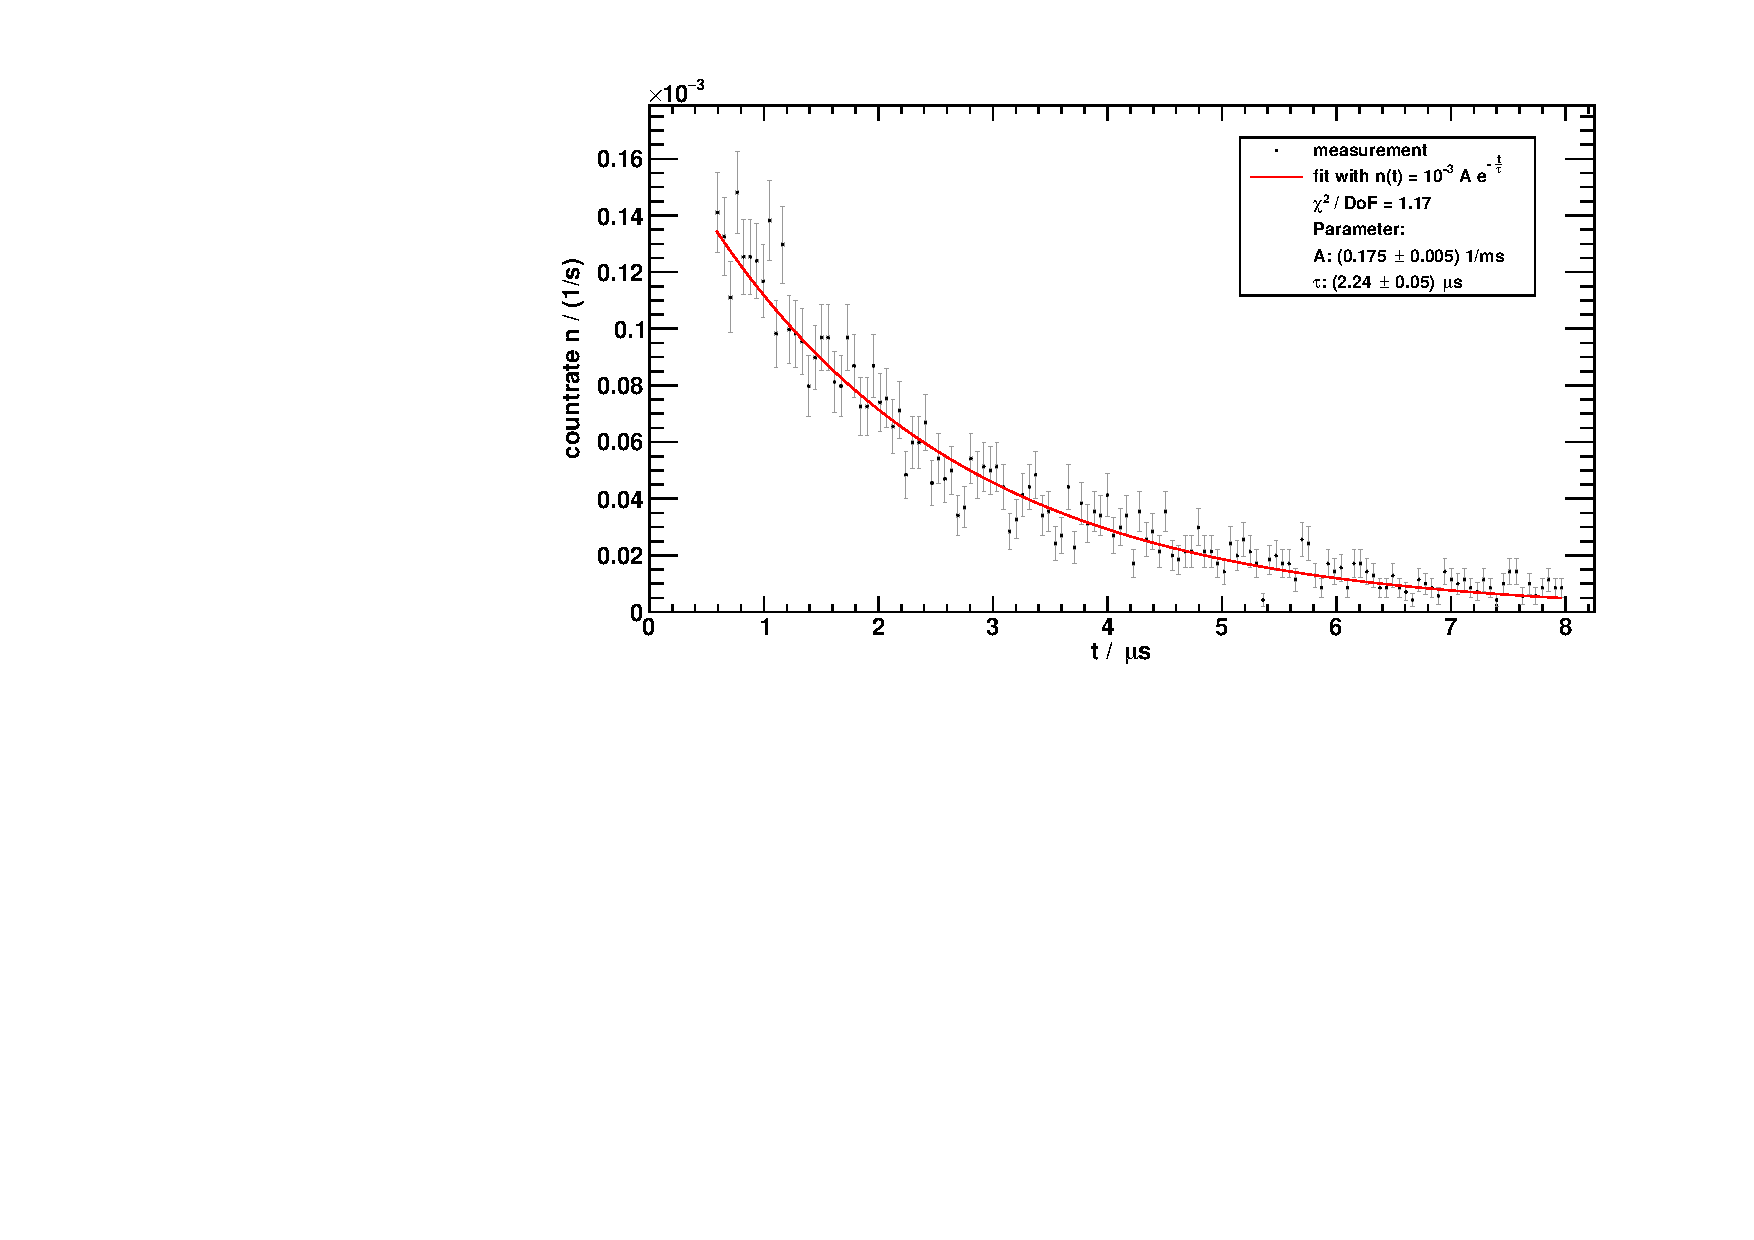
\includegraphics[width=\textwidth]{../img/decayTime.pdf}
  \caption{decay time, t-errors not visible.}
  \label{img:decaytime}
\end{center}
\end{figure}

The so obtained datapoints (\autoref{img:decaytime}) get fitted with an exponential function, since they obey the law of decay (\ref{sub:decay}):
\begin{equation}
    n = A \cdot e^{-\frac{t}{\tau}}
\end{equation}
The fit yields for the mean lifetime:
\begin{equation}
	\label{eq:result:meanlifetime}
    \tau = \left( 2.24 \pm 0.05 \right)\,\text{\textmu s}
\end{equation}
This matches with the literature value (\autoref{eq:litval:meanlifetime}) within 1-\textsigma-interval.
\begin{equation}
    \tau^{\text{lit.}} = \left( 2.1969811 \pm 0.0000022 \right)\,\text{\textmu s}
\end{equation}

\subsection{Weak coupling constant}
Now the weak coupling constant $G_\mu$ can be calculated with the muon's mass and mean lifetime. \autoref{eq:weakcouplingconstant} is used. The 
calculation is performed in natural units:
\begin{equation}
    \begin{split}
        G_\mu &= \sqrt{\frac{192 \pi^2}{\tau_\mu m_\mu^5}} \\
        s_{G_\mu} &= \frac{1}{2} \sqrt{\frac{192 \pi^3 \left( m_\mu^2 s_{\tau_\mu}^2 + 25 \tau_\mu^2 s_{m_\mu}^2 \right)}{m_\mu^7 \tau_\mu^3}}
    \end{split}
\end{equation}
With the relation
\begin{equation}
    t_\text{natural} = \frac{1}{\hbar} t_\text{S.I.}
\end{equation}
the mean lifetime can be converted to natural units. $\hbar$ has to be in eVs. \\
The weak coupling constant calculates to:
\begin{equation}
    G = (1.10 \pm 0.04) \cdot 10^{-5}\,\frac{1}{\text{GeV}^2}
\end{equation}
This result agrees with the literature value (\autoref{eq:litval:weakcouplingconstant}) within 1-\textsigma-interval.
\begin{equation}
    G_\mu^{\text{lit.}} = \left( 1.166364 \pm 0.000005 \right) \cdot 10^{-5}\,\frac{1}{\text{GeV}^2}
\end{equation}

%TODO add when finished
%\appendix
%\section{Anhang}
%\subsection{Messprotokoll}
%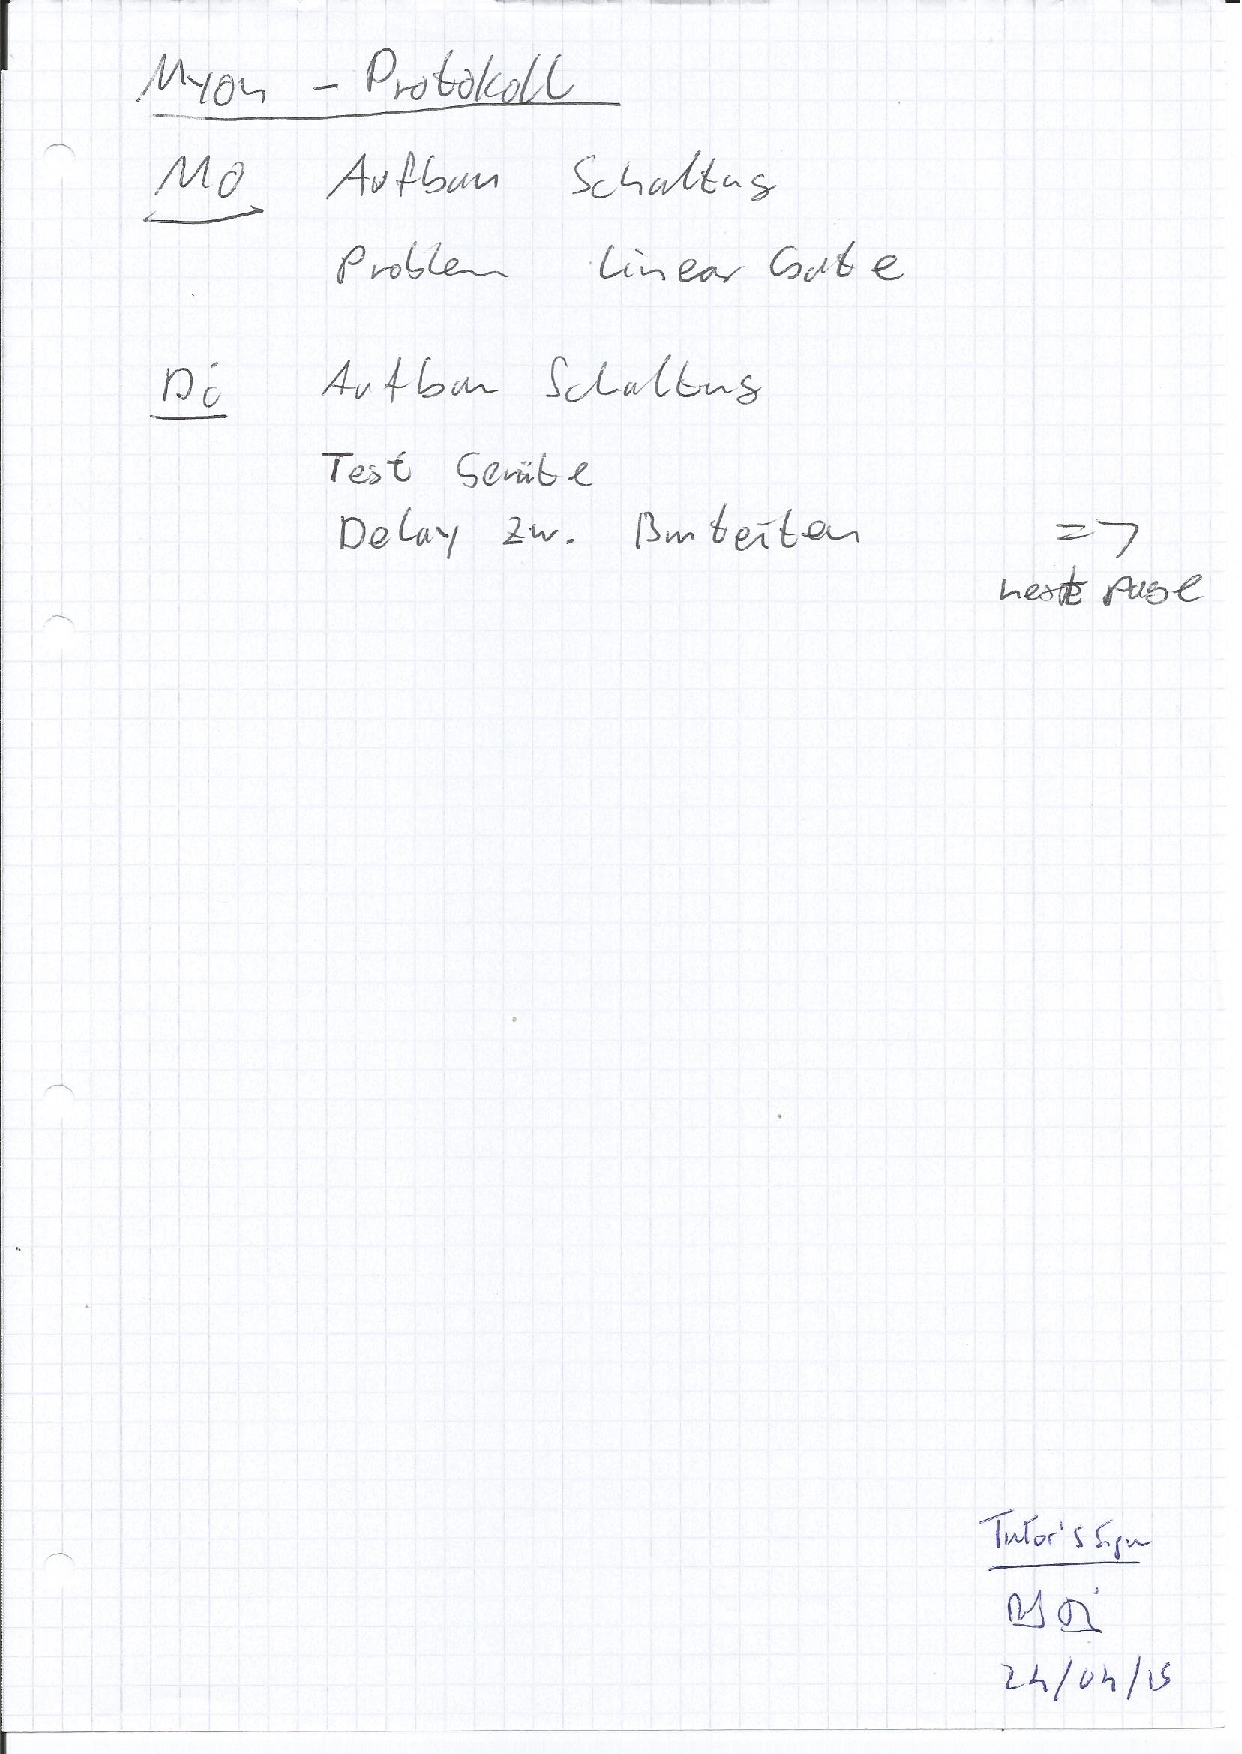
\includepdf[pages={-}]{../data/protokoll.pdf}


\end{document}